\chapter{Subcellular Localisation of Nascent IFIT Proteins in the Context of RSV Inclusion Bodies} \label{ch:Subcellular Localisation of Nascent IFIT Proteins in the Context of RSV Inclusion Bodies}
\section{Background and Aims} \label{sec:Background and Aims-Chapter3}
As elucidated in the preceding chapters, human \textit{IFIT} genes exhibit induction in response to both human and bovine RSV infections, suggesting their potential contribution to an anti-RSV role \textit{in vivo}. In contrast, the responsiveness of bovine \textit{IFITs} to human and bovine RSV infections appears limited, possibly influenced by baseline expression levels of these genes. Notably, Drori et al. reported that ectopically expressed human IFIT1, IFIT2, and IFIT3 hindered the growth of hRSV, though the precise mechanism of action remains elusive \cite{Drori2020InfluenzaProteins}. IFIT proteins, known for their diverse antiviral functions, engage in various mechanisms, differing among the IFIT proteins. These mechanisms include direct interactions of IFIT1 and IFIT5 with 5'-RNA modifications \cite{Abbas2013StructuralProteins, Diamond2014IFIT1:Translation}, IFIT2's pro-apoptotic action mediated through direct interactions with mitochondrial membranes \cite{Chen2017InhibitionApoptosis}, and IFIT3-mediated potentiation of RIG-I signaling via scaffold formation between MAVS and TBK1 on mitochondrial membranes \cite{Liu2011IFN-InducedTBK1}. Additionally, IFIT1, IFIT2, and IFIT3 form heterodimer and heterotrimer protein complexes, enhancing IFIT stability and potentially influencing their functions \cite{Mears2018BetterResponse}. Examining the subcellular localization of IFIT proteins in infected cells may serve as a proxy for understanding their mechanism of RSV inhibition. We propose that the sites of IFIT/RSV interactions are the RSV inclusion bodies, which form early in the infection cycle (6 HPI). These membraneless viral organelles, created by liquid-liquid phase separation, contain essential components of the RSV viral polymerase complex and serve as functional sites for RSV RNA transcription and replication \cite{Rincheval2017FunctionalVirus, Weber1995NonstructuralSerum, Fricke2013P38Assembly, Jobe2021BovineResponses}. IBs house the RNA genome and polyadenylated RNA, with the latter spatially segregated into substructures called IBAGs (IB-associated granules), while the genome is distributed throughout the IB structure but excluded from IBAGs \cite{Rincheval2017FunctionalVirus}. RSV IBs increase in size and complexity as they mature, with only larger, more mature IBs containing IBAGs \cite{Rincheval2017FunctionalVirus, Jobe2021BovineResponses}. IBAGs further contain the M2/1 protein, along with the eukaryotic translation initiation factors eIF4G, eIF4F, eIF3A, eIF4H, eIF4A, eIF4A1, and eIF4B \cite{Rincheval2017FunctionalVirus, Jobe2023ViralCondensates}. Given the reported interactions of IFIT1 and IFIT2 with eIF3E and eIF3C, hindering 43S-mRNA complex formation \cite{Diamond2014IFIT1:Translation, Guo2000CharacterizationVirus}, further indicating that the mechanism of action of these proteins against RSV could be mediated via IB interaction. Moreover, the maturation process of RSV IBs, characterized by increased size and complexity, with larger, mature IBs containing IBAGs, further underscores the potential significance of IFIT/IB interactions \cite{Rincheval2017FunctionalVirus, Jobe2021BovineResponses}. Our objective was to delineate the specific functions of IFIT proteins contributing to the reduction in RSV fitness. To achieve this, we initiated an assessment and comparison of the subcellular localization of human and bovine IFIT proteins under various conditions, including mock infection, treatment with human/bovine IFN\(\alpha\), and human/bovine RSV infection. Subsequently, we undertook a thorough analysis of human and bovine IFIT proteins, focusing on their interactions with the corresponding RSV IBs across multiple cell lines. These observations were made using confocal microscopy, allowing for a comprehensive exploration of the dynamic interactions between IFIT proteins and RSV IBs.

\section{Results} \label{sec:Results-Chapter3}
\subsection{IFIT Subcellular Localisation during Interferon Induction and RSV Infection} \label{subsec:IFIT Subcellular Localisation During Interferon Induction and RSV Infection}
A549, MDBK, and later BEAS2B cell lines were seeded on a 13 mm diameter glass coverslip in a 24-well plate at an initial concentration of 100,000 cells per well, as described in Section \ref{sec:Cell Culture}. 24 hours post-seeding, these cells were either mock-infected, treated with either human or bovine IFN$\upalpha$ at concentrations of 1,000 international units per mL for the former or 5 ng/mL for the latter (these concentrations are equivalent to each other), or infected with either human or bovine wild-type RSV at an MOI of 1. After 24 hours, the samples were fixed with paraformaldehyde and prepared as described in Section \ref{sec:Confocal Microscopy} for subsequent confocal microscopy analysis. The samples were stained with DAPI, allowing nuclear detection (consistently shown in yellow), antibodies against the RSV N protein (consistently shown in cyan), and the IFIT proteins (consistently shown in magenta). We initially assessed a panel of anti-IFIT antibodies, generously provided by the Viral Gene Expression Group at The Pirbright Institute. This panel included two antibodies for each of the human IFIT proteins, routinely employed for Western blotting by the group. In our confocal microscopy experiments, only one antibody per IFIT1, IFIT3, and IFIT5 yielded satisfactory results, while both antibodies against IFIT2 demonstrated efficacy. Consequently, we proceeded with single specific antibodies for IFIT1, IFIT3, and IFIT5, and utilised both IFIT2 antibodies, which we will refer to as IFIT2(A) and IFIT2(B) for simplicity.

Figure \ref{fig:Alterations in the Subcellular Localisation of Human IFITs in A549 Cells Exposed to hIFNa or hRSV} illustrates the subcellular localisation of human IFIT proteins in mock-, hIFN$\upalpha$-, or human RSV-treated samples observed in the A549 cell line. Human IFIT1 is primarily cytoplasmic and excluded from the nucleus in a basal state. Remarkably, hIFN$\upalpha$ stimulation does not alter this localisation pattern, and there is no discernible impact on the abundance of IFIT1, as evidenced by signal intensity. Throughout infection, IFIT1 maintains its cytoplasmic localisation, remaining excluded from the nucleus, potentially colocalising with N on the outer surface of the IB structure. The staining intensity exhibits an increase, particularly in uninfected cells, providing support for the hypothesis proposed in Chapter \ref{ch:Assessment of Transcriptional Induction of Human IFITs in the Context of RSV}—specifically, that RSV infection prophylactically induces IFIT expression in non-infected cells in an IFN-dependent manner. The IFIT2(A) antibody reveals hIFIT2 to be located in a cytoplasmic, diffused, but nuclearly excluded vesicular pattern in both basal and IFN$\upalpha$-induced states. The intensity between these two conditions appears equal. During hRSV infection, the overall intensity seems to decrease, and the localisation phenotype changes into a phenotype with fewer vesicles and inclusions inside the RSV IB structures. Conversely, the IFIT2(B) antibody detects IFIT2 to be granular and cytoplasmic, also depicting it as excluded from the nucleus. Similar to the IFIT2(A) antibody, the intensity and localisation phenotype between mock and IFN$\upalpha$ treated cells are equal. During hRSV infection, this antibody detects IFIT2 to be excluded from both the nucleus and the inclusion body, while retaining a vesicular cytoplasmic stain. IFIT3 appears to be cytoplasmic with nuclear exclusion under basal conditions. After IFN$\upalpha$ treatment, an increase in staining intensity and signs of IFIT3 nuclear translocation can be observed. During hRSV infection, IFIT3 seems to be evenly diffused throughout the whole cell, including the RSV inclusion body and the nucleus. The intensity of staining during infection appears similar between IFN$\upalpha$ treated and hRSV-infected cells. IFIT5 is also primarily cytoplasmically located under basal conditions while being excluded from the nucleus. During IFN$\upalpha$ treatment, the phenotype and intensity of the staining remain the same. During hRSV infection, an increase in IFIT5 levels is observed in uninfected cells. Regarding the staining pattern, it remains cytoplasmic and excluded from both the nucleus and RSV IB.

\begin{figure}
    \centering
    \includegraphics[width=1\linewidth]{08. Chapter 3/Figs/01. Localisation introduction/07. a549 merges.pdf}
    \caption[Alterations in the Subcellular Localisation of Human IFITs in A549 Cells Exposed to hIFN$\upalpha$ or hRSV.]{\textbf{Alterations in the Subcellular Localisation of Human IFITs in A549 Cells Exposed to hIFN$\upalpha$ or hRSV.} A549 cells underwent mock treatment, were treated with 1000 IU/mL of hIFN$\upalpha$ for 24 hours, or were infected with hRSV MOI 1 for 24 hours. Subsequently, cells were fixed and stained, using DAPI for nuclei detection (depicted in yellow), anti-RSV N antibody (shown in cyan), or antibodies targeting IFIT proteins (illustrated in magenta). Notably, two distinct antibodies against IFIT2 were utilised, designated as IFIT2(A) and IFIT2(B). Insets featuring magnified selections were generated from infected images, facilitating a clearer presentation of the underlying subcellular localisations.}
    \label{fig:Alterations in the Subcellular Localisation of Human IFITs in A549 Cells Exposed to hIFNa or hRSV}
\end{figure}

Figure \ref{fig:Modulations in the Subcellular Localisation of Bovine IFITs in MDBK Cells Exposed to bIFNa or bRSV} presents the subcellular localisation of bovine IFIT proteins in MDBK cell line under mock, bIFN$\upalpha$, or bovine RSV treatment conditions. Under basal conditions, bIFIT1 is primarily located in the cytoplasm with nuclear exclusion, accompanied by vesicles dispersed throughout cells, reminiscent of cytoplasmic bodies as classified by the Human Protein Atlas \cite{Thul2017AProteome}. Upon bIFN$\upalpha$ stimulation, the subcellular localisation remains unchanged, while the overall staining intensity increases. In samples infected with bRSV, cytoplasmic staining is observed with nuclear and IB exclusion, without apparent vesicles. Surrounding non-infected cells display an increased IFIT1 signal, while infected cells exhibit staining intensity lower than what was observed with interferon-stimulated cells. The IFIT2(A) antibody detects bIFIT2 predominantly in the cytoplasm, concentrated near the nucleus in a staining pattern resembling the Golgi apparatus, as classified by the Human Protein Atlas \cite{Thul2017AProteome}. This signal is also excluded from the nucleus. In interferon-treated cells, the overall pattern appears to be the same, with the exception of decreased staining intensity and decreased size of nuclearly proximal condensations. During bRSV infection, results are identical to what was observed in the A549 cell line, with the cytoplasmic signal greatly reduced. Instead, IFIT2 either colocalises with RSV N at the boundary of the IB or concentrates inside the inclusion bodies. IFIT2(B) shows bIFIT2 to be cytoplasmic with vesicles present throughout the cytoplasm and nucleus under basal conditions. It also appears to concentrate within the mitotic spindle, as classified by the Human Protein Atlas \cite{Thul2017AProteome}. Unfortunately, cells treated with bIFN$\upalpha$ and stained with IFIT2(B) antibody are lacking. During bRSV infection, this antibody shows bIFIT2 to have the same localisation and intensity as observed in mock cells. It also demonstrates IFIT2 to be excluded from the IB structure. bIFIT3 appears to be localised in vesicles with cytoplasmic and nuclear localisation in both mock and bIFN$\upalpha$ treated cells. The intensity signal appears slightly stronger in interferon-treated samples. During bRSV infection, IFIT3 subcellular localisation changes drastically. It is barely detectable in the cytoplasm and nucleus, except for strong intra-IB inclusions. There also appear to be vesicles inside the inclusion that resemble the IBAGs. bIFIT5 shows cytoplasmic localisation with vesicles diffused through the cytoplasm, weak nuclear staining, and inclusions within nucleoli. In samples treated with bIFN$\upalpha$, although the pattern of subcellular localisation remains the same, the intensity increases, especially in the nucleus. Finally, in cells infected with bRSV, nuclear exclusion occurs with inclusion within the nucleoli, and cytoplasmic staining with no clear colocalisation or exclusion with RSV IBs. The observed cytoplasmic vesicles are only evident in non-infected cells. The intensity of the staining resembles that of mock-treated cells.

\begin{figure}
    \centering
    \includegraphics[width=1\linewidth]{08. Chapter 3/Figs/01. Localisation introduction/09. mdbk-merges-test.pdf}
    \caption[Modulations in the Subcellular Localisation of Bovine IFITs in MDBK Cells Exposed to bIFN$\upalpha$ or bRSV.]{\textbf{Modulations in the Subcellular Localisation of Bovine IFITs in MDBK Cells Exposed to bIFN$\upalpha$ or bRSV.} MDBK cells underwent either mock treatment, exposure to 5 ng/mL of bIFN$\upalpha$ for 24 hours, or infection with bRSV MOI 1 for 24 hours. Subsequently, cells were fixed and stained using DAPI for nuclei detection (depicted in yellow), anti-RSV N antibody (shown in cyan), or antibodies targeting IFIT proteins (illustrated in magenta). Notably, two distinct antibodies against IFIT2 were employed, referred to as IFIT2(A) and IFIT2(B). Insets featuring magnified selections were derived from infected images, facilitating a clearer presentation of the underlying subcellular localisations.}
    \label{fig:Modulations in the Subcellular Localisation of Bovine IFITs in MDBK Cells Exposed to bIFNa or bRSV}
\end{figure}

We can observe a wide variety of subcellular localisations and interactions with the RSV inclusion bodies when these results are considered collectively. Notably, a consistent observation across cell lines and IFITs is the infrequent occurrence of changes in localisations due to IFN$\upalpha$ stimulation. Instead, it predominantly results in an increased concentration or no discernible difference compared to mock-treated samples. A noteworthy exception is the increased nuclear localisation observed in human IFIT3 and the altered pattern in bovine IFIT2, as detected by the IFIT2(A) antibody, showcasing a decreased overall signal and a modified Golgi apparatus-like staining pattern. Human and bovine IFIT1 exhibit cytoplasmic localisation with nuclear exclusion. During infection, both seem to be more expressed in uninfected cells. Bovine IFIT1, in particular, displays the presence of cytoplasmic vesicles and differential interaction with IBs, being excluded, while human IFIT1 appears to colocalise with the IB boundary. The IFIT2 antibodies provide distinct outcomes concerning the detected interaction of IFIT2 with IBs, while maintaining consistent results across human and bovine cell lines. IFIT2(A) antibody demonstrates the interaction of human and bovine IFIT2 with RSV IBs, with human IFIT2 forming intra-IB inclusions and bovine IFIT2 colocalising with the IB boundary. In contrast, IFIT2(B) consistently detects the exclusion of IFIT2 from IBs in both cell lines. Discrepancies are observed in basal localisation, both between antibodies and cell lines. In human cells, IFIT2(A) is vesicular, while IFIT2(B) exhibits a more granular cytoplasmic stain. In bovine cells, IFIT2(A) shows cytoplasmic staining with IFIT2 concentrations proximal to the nucleus, and IFIT2(B) displays a vesicular stain without these structures. Further investigation is necessary to elucidate the differential staining patterns observed with the two polyclonal antibodies. We hypothesise that these antibodies may be targeting two distinct IFIT2 epitopes. Possibilities include detection of its monomeric or dimeric state, identification of IFIT2 in complex with its interaction partners, or recognition of an unfamiliar antigenic state that requires further elucidation. Differential IFIT3 signals are noted between human and bovine cells, both in basal localisation and interaction with RSV IBs. Human IFIT3 is cytoplasmic and nuclearly excluded under basal conditions, with nuclear translocation after stimulation with either IFN$\upalpha$ or hRSV. In contrast, bovine IFIT3 is vesicular with nuclear staining under basal conditions, but nuclear staining disappears in bRSV-infected cells. Regarding RSV IB interaction, human IFIT3 is diffused evenly throughout the cytoplasm, nucleus, and IB structures, while bovine IFIT3 forms intra-IB inclusions with signs of IBAGs. Small differences are also observed between human and bovine IFIT5 staining. Both are basally cytoplasmic, with increased intensity after IFN$\upalpha$ stimulation. Bovine IFIT5 is additionally observed in cytoplasmic vesicles, nuclei, and intra-nucleolar inclusions. During infection, both human and bovine IFIT5 exhibit cytoplasmic and nuclear exclusion, with bovine IFIT5 retaining the intra-nucleolar inclusion. Regarding the interaction with RSV IBs, human IFIT5 was evidently excluded, whereas we faced challenges in definitively determining the bovine IFIT5 interaction phenotype with bovine RSV IBs.

In light of the potentially interesting findings concerning the colocalisation of IFITs with RSV IBs, we expanded our investigation with hRSV infections in the BEAS2B cell line. A comprehensive analysis was conducted, systematically examining 1727 IB sizes and their underlying interaction phenotypes with various IFIT proteins. The phenotypic categorisation was based solely on IFIT staining in regions where the presence of IBs was confirmed by viral nucleoprotein staining. Figure \ref{fig:Inclusion Bodies Within RSV Infected Cells: Zoom Sequence} illustrates a representative region of interest, showcasing its location within the cell and the broader cellular population. Based on our observations, we classified the phenotypes as follows: \textbf{Diffusion} phenotype was assigned when the IFIT signal spread equally across the area of interest; \textbf{Exclusion} phenotype was designated by an obvious, partial, or complete decrease in signal within the IB boundary; \textbf{Edge Exclusion} phenotype was assigned when the IFIT signal spread uniformly across the area of interest, except for exclusion from the IB boundary; \textbf{Inclusion} phenotype was attributed to a clear increase in the IFIT signal within the IB boundary; and \textbf{Colocalisation} phenotype was assigned when the IFIT signal spread uniformly across the area of interest, except for an increased signal in the IB boundary. Additionally, these main phenotypes were sometimes complemented by either their interaction or the presence of spots within the IB boundary. Notably, a common occurrence was colocalisation accompanied by exclusion, indicating a marked increase on the IB boundary compared to the surrounding signal, alongside a noticeable decrease within the region of interest. For the former, these spots are hypothesised to represent the inclusion body-associated granules (IBAGs). The frequency of occurrence of these phenotypes was calculated, and an arbitrary cutoff of 5\% was established to distinguish phenotypes that, due to their low frequency, were considered not relevant in the context of RSV infection.

\begin{figure}
    \centering
    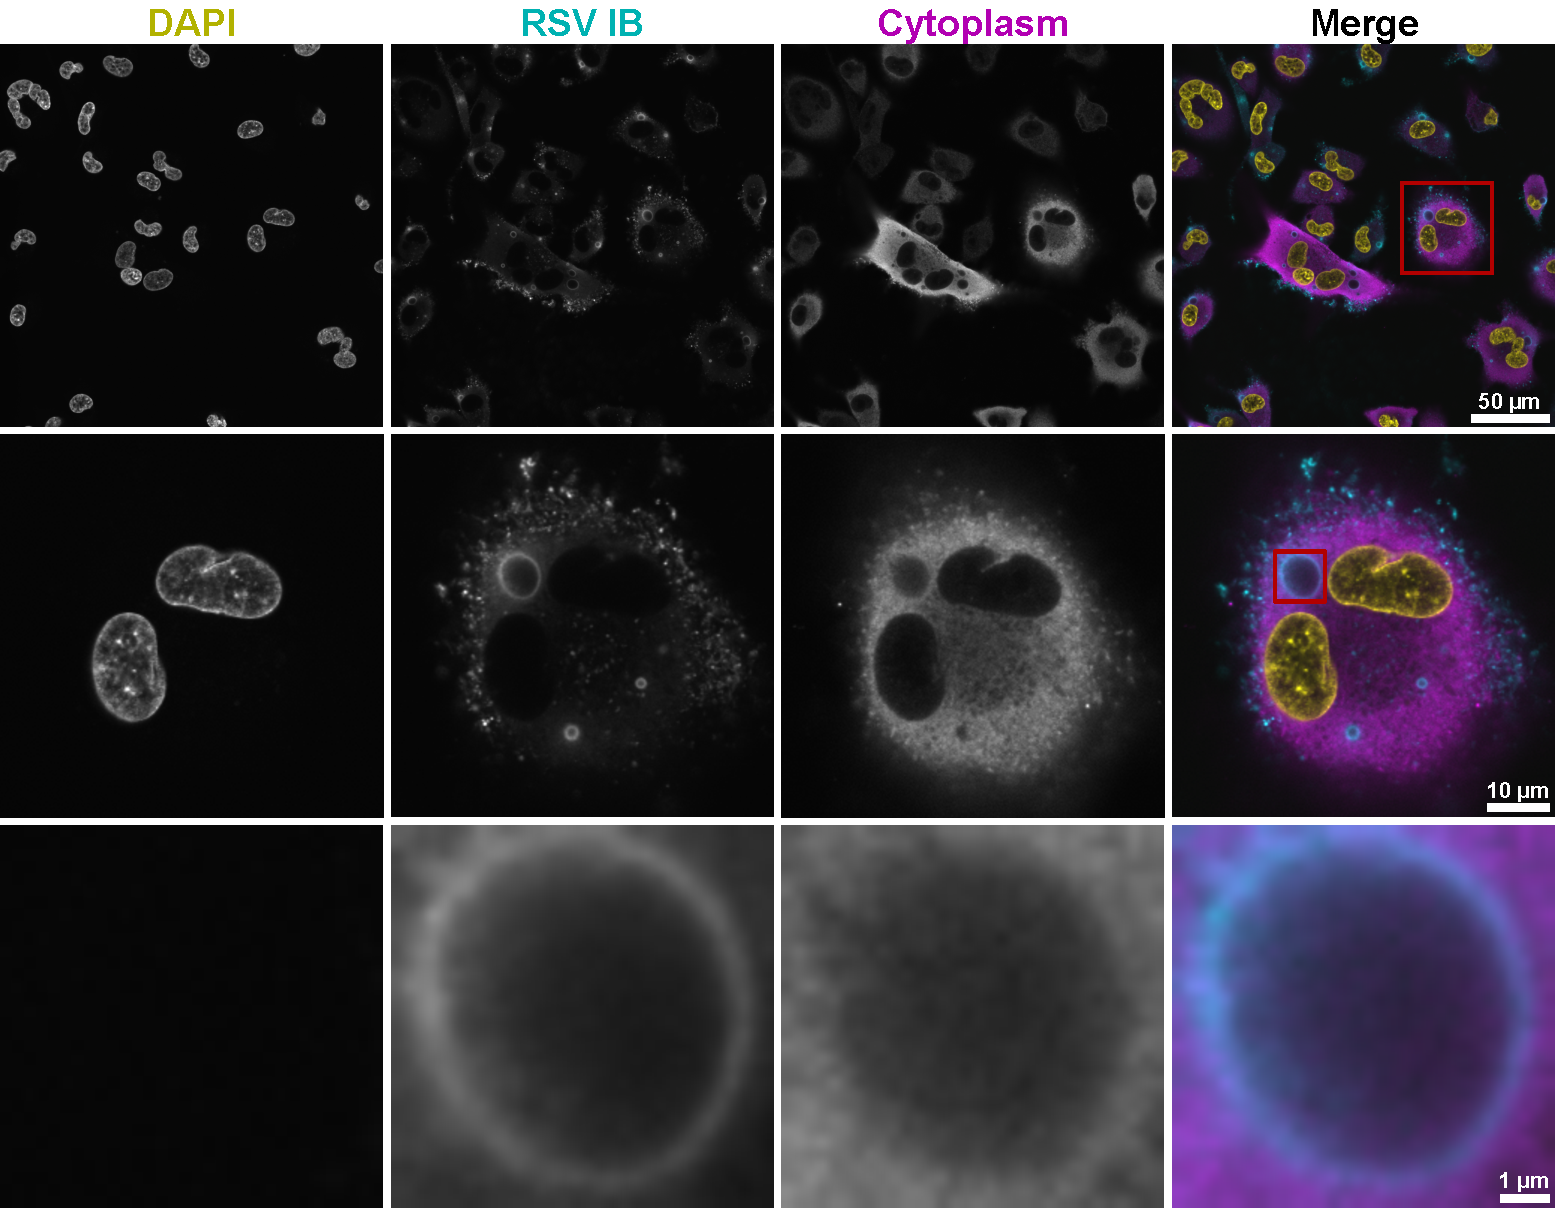
\includegraphics[width=1\linewidth]{08. Chapter 3/Figs/01. Localisation introduction/01. IB-zooms.pdf}
    \caption[Inclusion Bodies Within RSV-Infected Cells: Zoom Sequence.]{\textbf{Inclusion Bodies Within RSV-Infected Cells: Zoom Sequence.} A representative image of RSV-infected cells detected using confocal microscopy. Cellular nuclei were stained with DAPI and are depicted in yellow; RSV inclusion bodies, stained for RSV P, are represented in cyan; and the cytoplasm, stained for IFIT5, is illustrated in magenta. The figure showcases a zoom sequence starting from a population of cells, progressing to a single syncytial view, and ultimately focusing on an individual inclusion body.}
    \label{fig:Inclusion Bodies Within RSV Infected Cells: Zoom Sequence}
\end{figure}

We systematically observed and annotated a total of 1727 inclusion bodies across different cell lines, categorising their IFIT interaction phenotypes and measuring their radii (µm) and areas (\(\mbox{µm}^2\)) based on the observed 2D projections. Specifically, we analysed 1008 hRSV IBs in the A549 cell line, 99 hRSV IBs in the BEAS2B cell line, and 620 bRSV IBs in the MDBK cell line. Figure \ref{fig:Size Characterization of Inclusion Bodies Observed Across Different Cell Lines} illustrates the relationship between IB area and radius, both as an aggregate of all observed IBs and IBs detected per cell line. The data, in both the aggregate and individual cell line view, broadly follows a logarithmic curve, indicating the predominant circular shape of the majority of IBs. However, a deviation from this pattern is noticeable in each cell line, particularly in larger IBs, where the area increases disproportionately with the radius, suggesting a more elongated ellipsoid shape. Most IBs, irrespective of their origin, conform to areas below 10 \(\mbox{µm}^2\). Regarding the most common radii, both BEAS2B and MDBK IBs tend to be below 1 µm, while A549 IBs exhibit a range of the most common radii sizes between 0.5 and 1.5 µm. A more detailed view of the distribution of measured areas per cell line can be observed in Figure \ref{fig:The Distributions of IB Areas Observed Per Cell Line}. Here, all three cell lines encompass IBs ranging from sub 0.5 \(\mbox{µm}^2\) to supra 30 \(\mbox{µm}^2\), with median sizes of 5 \(\mbox{µm}^2\), 3 \(\mbox{µm}^2\), and 2 \(\mbox{µm}^2\) for A549, BEAS2B, and MDBK, respectively. MDBK has the highest number of sub 1 \(\mbox{µm}^2\) IBs, while A549 exhibits the most supra 10 \(\mbox{µm}^2\) IBs.

\begin{figure}
    \begin{subfigure}{0.495\textwidth}
        \caption{}
        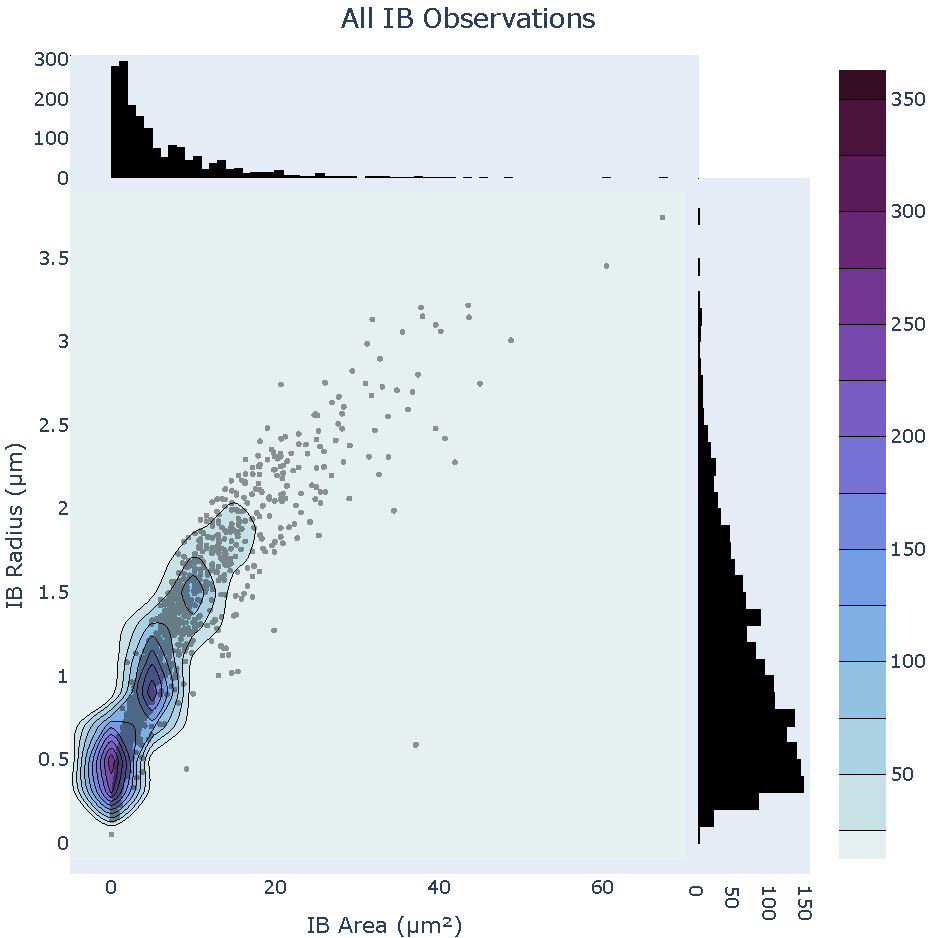
\includegraphics[width=\textwidth]{08. Chapter 3/Figs/01. Localisation introduction/02. heatmap_all.pdf} 
    \end{subfigure}
    \hfill
    \begin{subfigure}{0.495\textwidth}
        \caption{}
        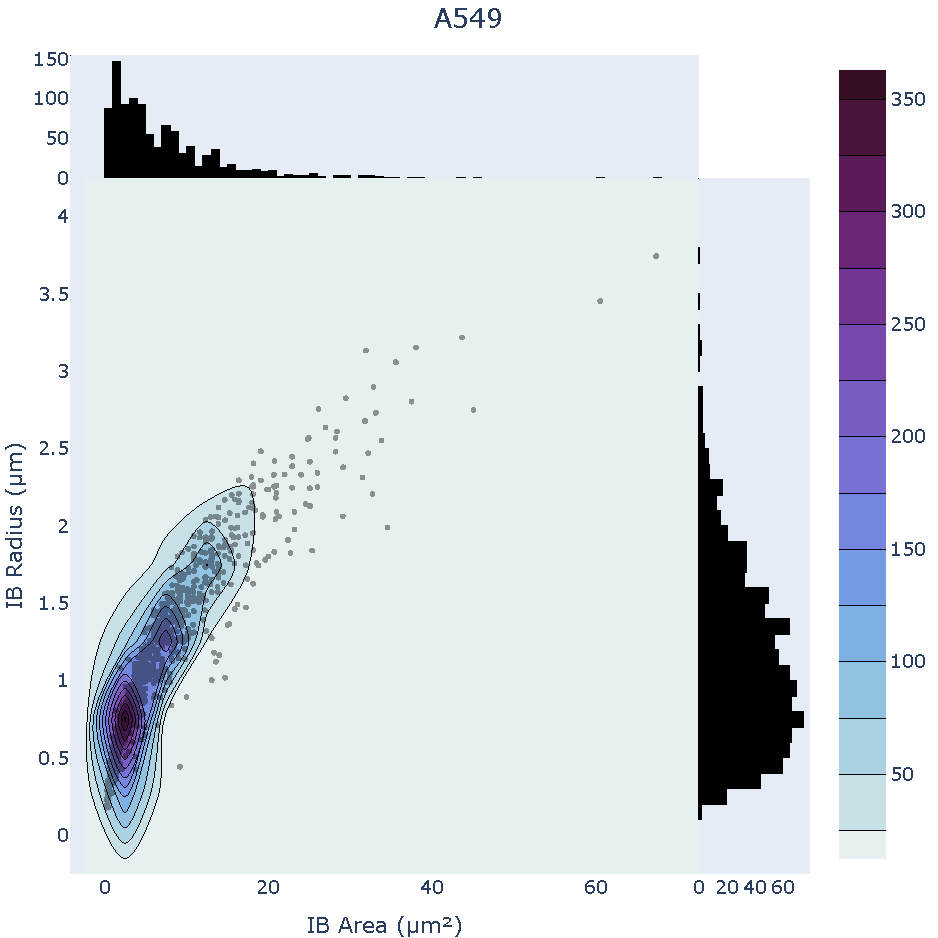
\includegraphics[width=\textwidth]{08. Chapter 3/Figs/01. Localisation introduction/03. heatmap_a549.pdf}
    \end{subfigure}

    \medskip
    \begin{subfigure}{0.495\textwidth}
        \caption{}
        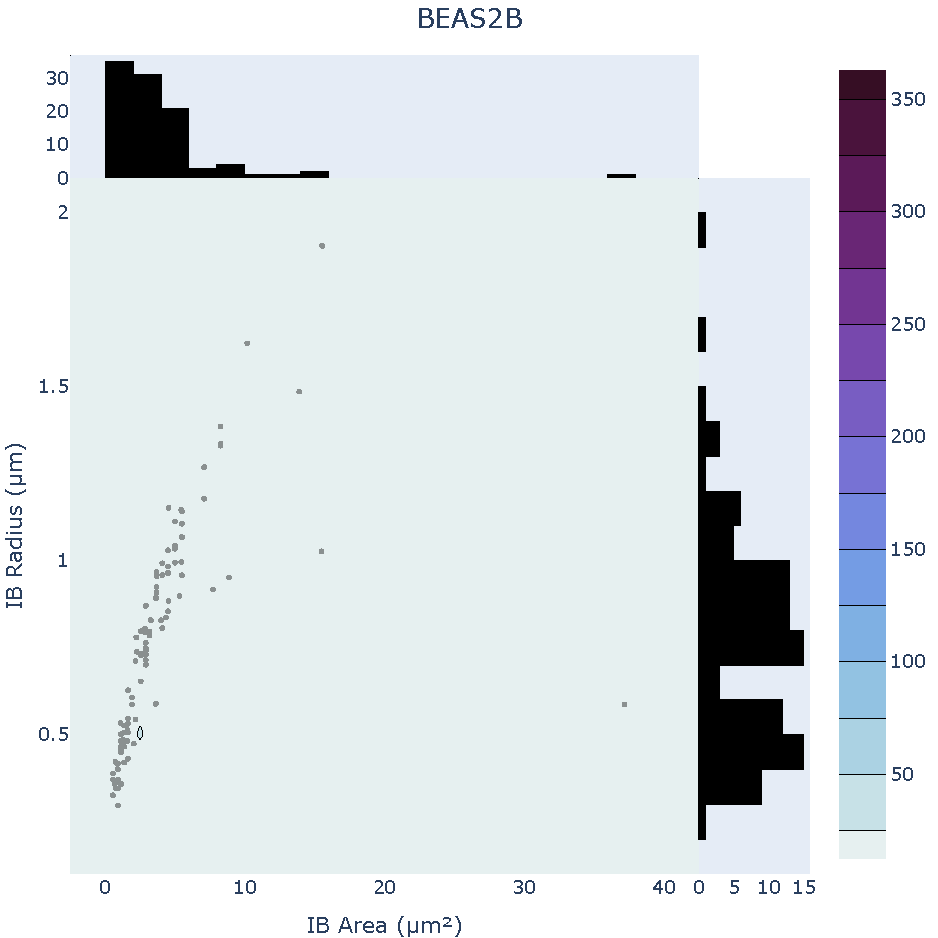
\includegraphics[width=\textwidth]{08. Chapter 3/Figs/01. Localisation introduction/04. heatmap_beas2b.pdf} 
    \end{subfigure}
    \hfill
    \begin{subfigure}{0.495\textwidth}
        \caption{}
        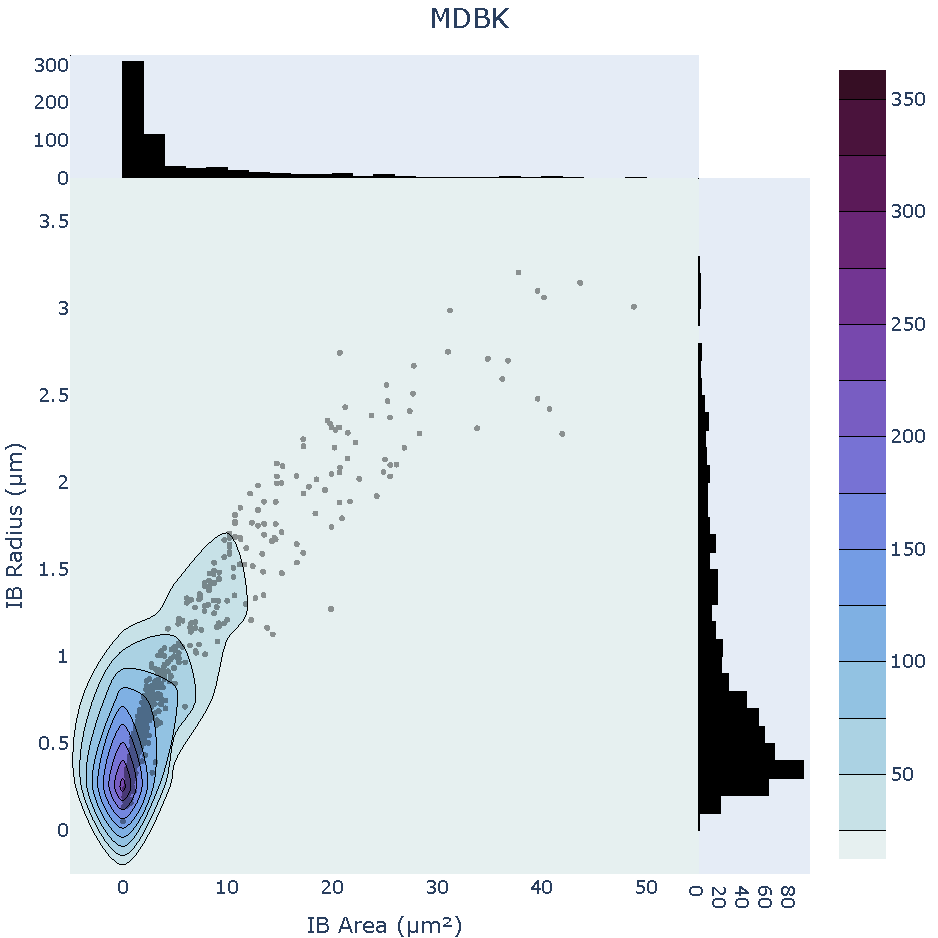
\includegraphics[width=\textwidth]{08. Chapter 3/Figs/01. Localisation introduction/05. heatmap_mdbk.pdf} 
    \end{subfigure}
    \caption[Size Characterisation of Inclusion Bodies Observed Across Different Cell Lines.]{\textbf{Size Characterisation of Inclusion Bodies Observed Across Different Cell Lines.} This figure elucidates the relationship between the measured area (\(\mbox{µm}^2\)) and radius (µm) of individual RSV inclusion bodies observed in this study. The figure includes distinct population distributions alongside the plots: (a) an aggregate of 1727 IB observations across all cell lines, (b) 1008 observations from the A549 cell line, (c) 99 observations from the BEAS2B cell line, and (d) 620 observations from the MDBK cell line. Contour plots are incorporated to highlight the density of individual IBs within the plots.}
    \label{fig:Size Characterization of Inclusion Bodies Observed Across Different Cell Lines}
\end{figure}

From the published literature, it is established that an increase in IB area correlates with its maturation state and internal complexity. Notably, in the HEp-2 cell line infected with hRSV, it has been reported that IBs containing IBAGs are significantly larger than those without (6.4 \(\mbox{µm}^2\) versus 2.3 \(\mbox{µm}^2\)) \cite{Rincheval2017FunctionalVirus}. Additionally, in the MDBK cell line, during the early infection timepoint (6 hours post-infection), only small IBs are present, with a mean area value of 1 \(\mbox{µm}^2\), and these do not contain IBAGs. At 16 hours post-infection, IBs without IBAGs retain the mean area value, while larger IBs with IBAGs (mean area of 10 \(\mbox{µm}^2\)) are also observed \cite{Jobe2021BovineResponses}. Importantly, at 24 HPI, a critical timepoint for the analysis in this thesis, small IBs without IBAGs maintain a median size of 1 \(\mbox{µm}^2\), while larger IBs containing IBAGs cluster into two sizes, with mean areas of 2.5 \(\mbox{µm}^2\) and 17 \(\mbox{µm}^2\). Based on this information, we can assess the observed IFIT-IB interaction phenotypes per mature or immature IBs.

\begin{figure}
    \centering
    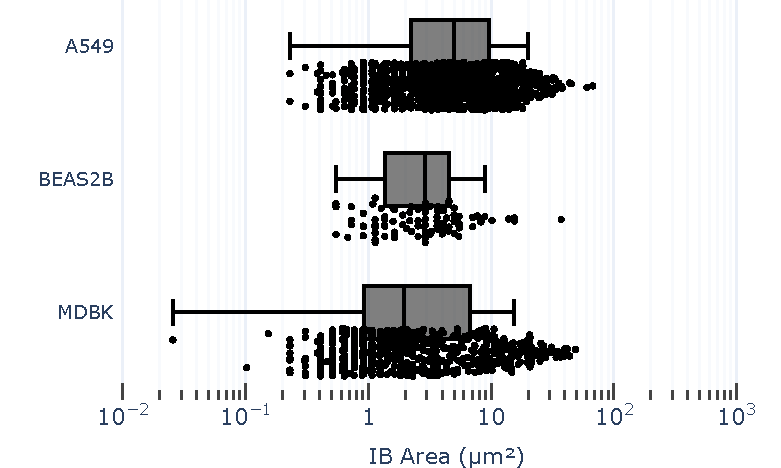
\includegraphics[width=1\linewidth]{08. Chapter 3/Figs/01. Localisation introduction/06. box-infection.pdf}
    \caption[The Distributions of IB Areas Observed per Cell Line.]{\textbf{The Distributions of IB Areas Observed per Cell Line.} The distribution of RSV inclusion body areas (\(\mbox{µm}^2\)), detected in this study are shown. A total of 1008 observations were made in the A549 cell line, 99 observations in the BEAS2B cell line, and 620 observations in the MDBK cell line.}
    \label{fig:The Distributions of IB Areas Observed Per Cell Line}
\end{figure}
\subsection{Nascent Human and Bovine IFIT Localisation During RSV Infection} \label{subsec:Nascent Human and Bovine IFIT Localisation During RSV Infection}
\subsubsection{Phenotypic Diversity of Nascent IFIT1 Interaction with RSV Inclusion Bodies}
following a hint of interaction with ibs for some ifits, we went to systematically assess the interaction of all ifits

ifit one, although being predominantly excluded or duffuesd through ibs (suggesting no interaction), is often observed to interact with these structures

inclusion and coloc + eclusion happens in larger ibs (probs more mature), suggesting temporal nature of ifit one interaction

30 excl 30 diff 18 incl 9 coloc + excl 9 edge excl
5, 4.4, 8, 12, 7

\lipsum[1-30]
\begin{figure}
    \begin{subfigure}{0.495\textwidth}
        \caption{}
        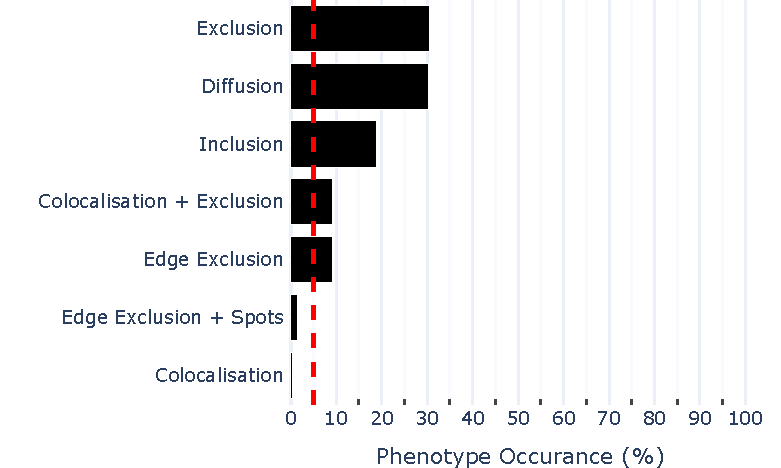
\includegraphics[width=1\linewidth]{08. Chapter 3/Figs/02. Infection/01. IFIT1/01. bar_i1_a549.pdf} 
    \end{subfigure}
    \begin{subfigure}{0.495\textwidth}
        \caption{}
        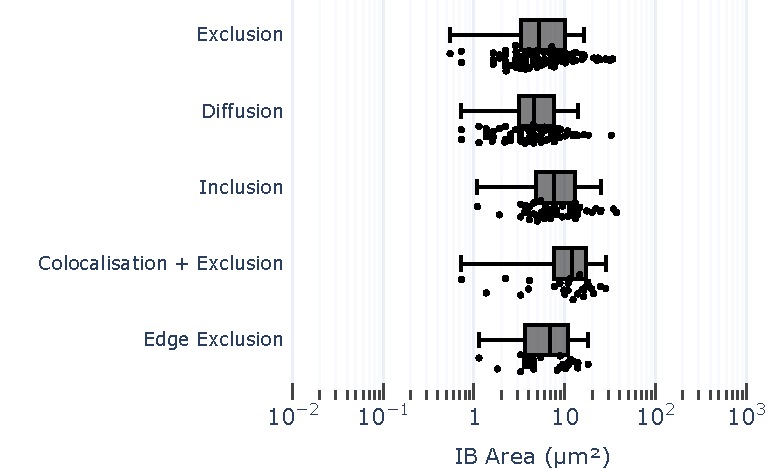
\includegraphics[width=1\linewidth]{08. Chapter 3/Figs/02. Infection/01. IFIT1/02. box_i1_a549.pdf}
    \end{subfigure}
    \caption[Phenotypic Diversity of hIFIT1 Interactions with hRSV Inclusion Bodies in A549 Cell Line.]{\textbf{Phenotypic Diversity of hIFIT1 Interactions with hRSV Inclusion Bodies in A549 Cell Line.} A549 cells were infected with human RSV at MOI 1 and fixed 24 HPI. Cells were double-labeled with with anti-RSV N and anti-IFIT1 antibodies and imaged on confocal microscope. Panel (a) shows percentual proportions of observed phenotypes between hRSV inclusion bodies and hIFIT1 (281 observations), with the red dotted line denoting the 5\% threshold, marking phenotypes considered relevant above this limit. Panel (b) shows the IB area in \(\mu m^2\) per observed relevant phenotype.}
    \label{fig:Phenotypic Diversity of hIFIT1 Interactions with hRSV Inclusion Bodies in A549 Cell Line}
\end{figure}

\begin{figure}
    \centering
    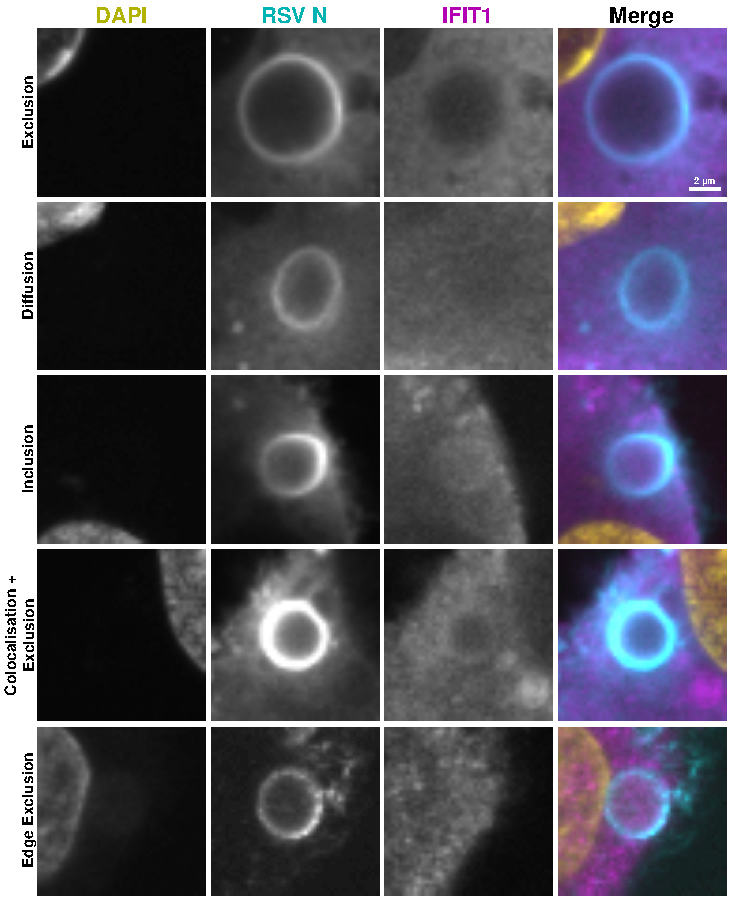
\includegraphics[width=1\linewidth]{08. Chapter 3/Figs/02. Infection/01. IFIT1/03. a549 i1.pdf}
    \caption[Representative Images of Phenotypic Diversity of hIFIT1 Interactions with hRSV Inclusion Bodies in A549 Cell Line.]{\textbf{Representative Images of Phenotypic Diversity of hIFIT1 Interactions with hRSV Inclusion Bodies in A549 Cell Line.} A549 cells were infected with hRSV at MOI 1 and fixed at 24 HPI. Cellular nuclei were stained with DAPI (yellow), and cells were double-labeled with anti-RSV N (cyan) and anti-IFIT1 (magenta) antibodies. This figure showcases representative examples of relevant phenotypes in the interaction between hIFIT1 and hRSV inclusion bodies. These phenotypes are presented in descending order based on their percentage proportions. The scale bar indicates 2 \(\mu m\).}
    \label{fig:Representative Images of Phenotypic Diversity of hIFIT1 Interactions with hRSV Inclusion Bodies in A549 Cell Line}
\end{figure}

in beas2bs there is mainly exclsion 86\% with some diffusion 8\%.

diffusion happens in smaller ibs 0.5 (compared to 3)

\begin{figure}
    \begin{subfigure}{0.495\textwidth}
        \caption{}
        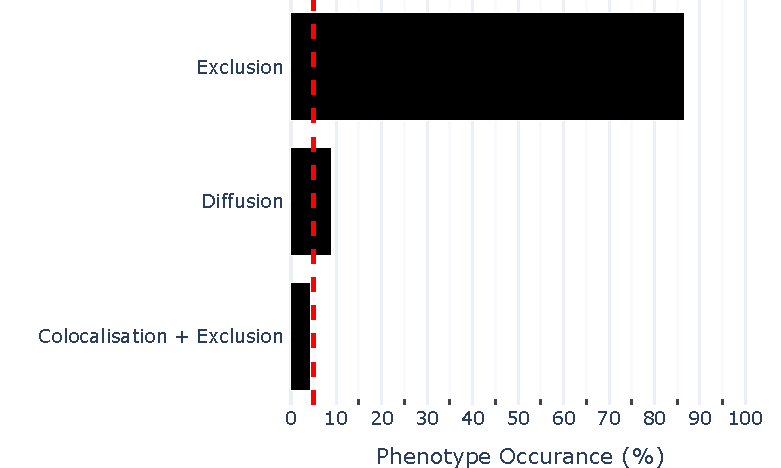
\includegraphics[width=1\linewidth]{08. Chapter 3/Figs/02. Infection/01. IFIT1/04. bar_i1_beas2b.pdf} 
    \end{subfigure}
    \begin{subfigure}{0.495\textwidth}
        \caption{}
        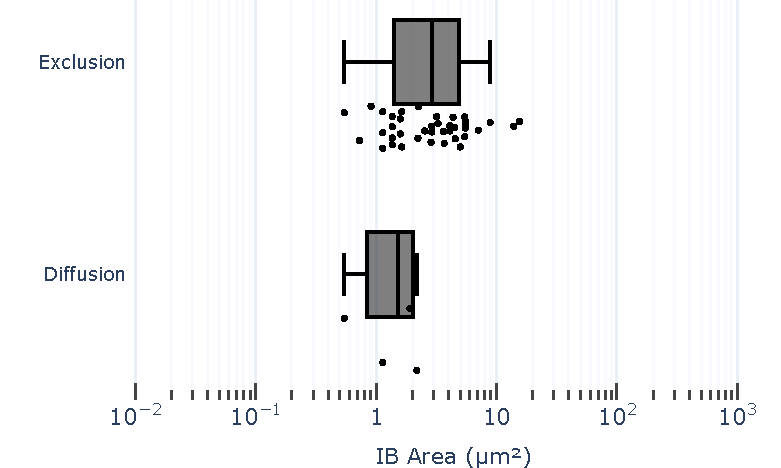
\includegraphics[width=1\linewidth]{08. Chapter 3/Figs/02. Infection/01. IFIT1/05. box_i1_beas2b.pdf}
    \end{subfigure}
    \caption[Phenotypic Diversity of hIFIT1 Interactions with hRSV Inclusion Bodies in BEAS2B Cell Line.]{\textbf{Phenotypic Diversity of hIFIT1 Interactions with hRSV Inclusion Bodies in BEAS2B Cell Line.} BEAS2B cells were infected with human RSV at MOI 1 and fixed 24 HPI. Cells were double-labeled with with anti-RSV N and anti-IFIT1 antibodies and imaged on confocal microscope. Panel (a) shows percentual proportions of observed phenotypes between hRSV inclusion bodies and hIFIT1 (281 observations), with the red dotted line denoting the 5\% threshold, marking phenotypes considered relevant above this limit. Panel (b) shows the IB area in \(\mu m^2\) per observed relevant phenotype.}
    \label{fig:Phenotypic Diversity of hIFIT1 Interactions with hRSV Inclusion Bodies in BEAS2B Cell Line}
\end{figure}

\begin{figure}
    \centering
    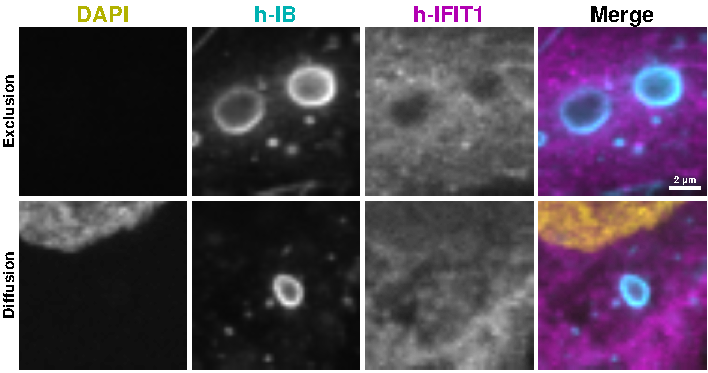
\includegraphics[width=1\linewidth]{08. Chapter 3/Figs/02. Infection/01. IFIT1/06. beas2b i1.pdf}
    \caption[Representative Images of Phenotypic Diversity of hIFIT1 Interactions with hRSV Inclusion Bodies in BEAS2B Cell Line.]{\textbf{Representative Images of Phenotypic Diversity of hIFIT1 Interactions with hRSV Inclusion Bodies in BEAS2B Cell Line.} BEAS2B cells were infected with hRSV at MOI 1 and fixed at 24 HPI. Cellular nuclei were stained with DAPI (yellow), and cells were double-labeled with anti-RSV N (cyan) and anti-IFIT1 (magenta) antibodies. This figure showcases representative examples of relevant phenotypes in the interaction between hIFIT1 and hRSV inclusion bodies. These phenotypes are presented in descending order based on their percentage proportions. The scale bar indicates 2 \(\mu m\).}
    \label{fig:Representative Images of Phenotypic Diversity of hIFIT1 Interactions with hRSV Inclusion Bodies in BEAS2B Cell Line}
\end{figure}

66 excl, 23 incl, 5 diff

2, 1, 1.5

\begin{figure}
    \begin{subfigure}{0.495\textwidth}
        \caption{}
        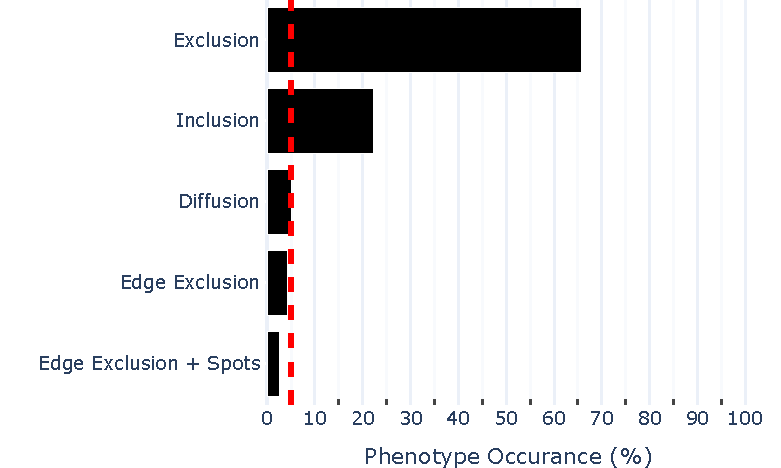
\includegraphics[width=1\linewidth]{08. Chapter 3/Figs/02. Infection/01. IFIT1/07. bar_i1_mdbk.pdf} 
    \end{subfigure}
    \begin{subfigure}{0.495\textwidth}
        \caption{}
        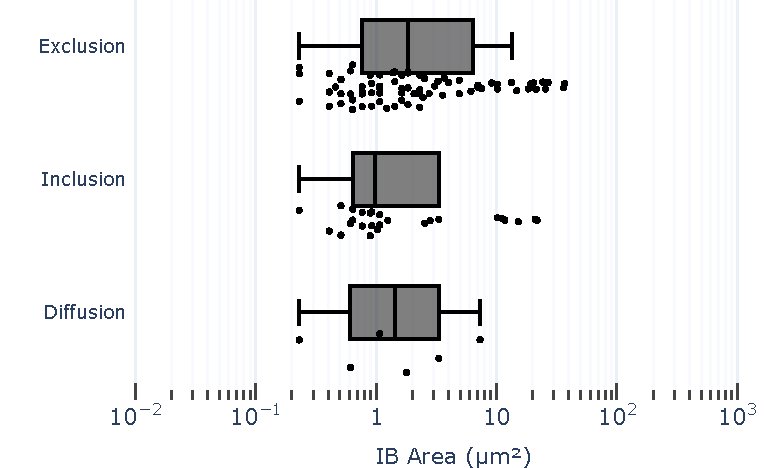
\includegraphics[width=1\linewidth]{08. Chapter 3/Figs/02. Infection/01. IFIT1/08. box_i1_mdbk.pdf}
    \end{subfigure}
    \caption[Phenotypic Diversity of bIFIT1 Interactions with bRSV Inclusion Bodies in MDBK Cell Line.]{\textbf{Phenotypic Diversity of bIFIT1 Interactions with bRSV Inclusion Bodies in MDBK Cell Line.} MDBK cells were infected with bovine RSV at MOI 1 and fixed 24 HPI. Cells were double-labeled with with anti-RSV N and anti-IFIT1 antibodies and imaged on confocal microscope. Panel (a) shows percentual proportions of observed phenotypes between bRSV inclusion bodies and bIFIT1 (117 observations), with the red dotted line denoting the 5\% threshold, marking phenotypes considered relevant above this limit. Panel (b) shows the IB area in \(\mu m^2\) per observed relevant phenotype.}
    \label{fig:Phenotypic Diversity of bIFIT1 Interactions with bRSV Inclusion Bodies in MDBK Cell Line}
\end{figure}

\begin{figure}
    \centering
    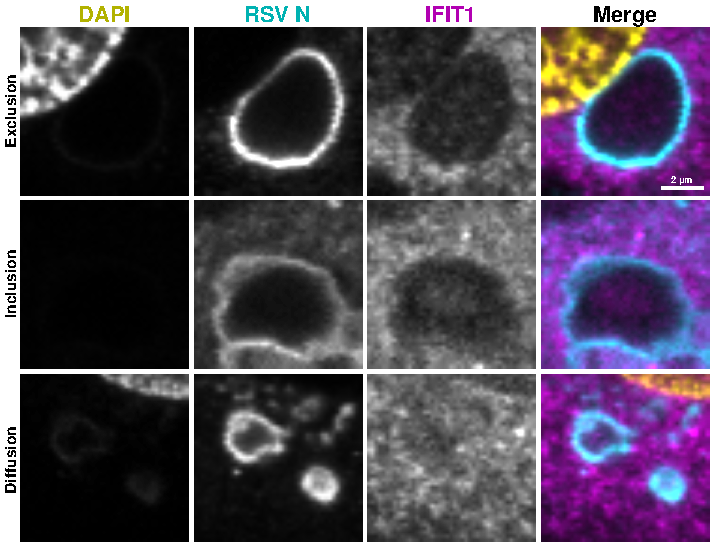
\includegraphics[width=1\linewidth]{08. Chapter 3/Figs/02. Infection/01. IFIT1/09. mdbk i1.pdf}
    \caption[Representative Images of Phenotypic Diversity of bIFIT1 Interactions with bRSV Inclusion Bodies in MDBK Cell Line.]{\textbf{Representative Images of Phenotypic Diversity of bIFIT1 Interactions with bRSV Inclusion Bodies in MDBK Cell Line.} MDBK cells were infected with bRSV at MOI 1 and fixed at 24 HPI. Cellular nuclei were stained with DAPI (yellow), and cells were double-labeled with anti-RSV N (cyan) and anti-IFIT1 (magenta) antibodies. This figure showcases representative examples of relevant phenotypes in the interaction between bIFIT1 and bRSV inclusion bodies. These phenotypes are presented in descending order based on their percentage proportions. The scale bar indicates 2 \(\mu m\).}
    \label{fig:Representative Images of Phenotypic Diversity of bIFIT1 Interactions with bRSV Inclusion Bodies in MDBK Cell Line}
\end{figure}

\subsubsection{Phenotypic Diversity of Nascent IFIT2 Interaction with RSV Inclusion Bodies}

\begin{figure}
    \begin{subfigure}{0.495\textwidth}
        \caption{}
        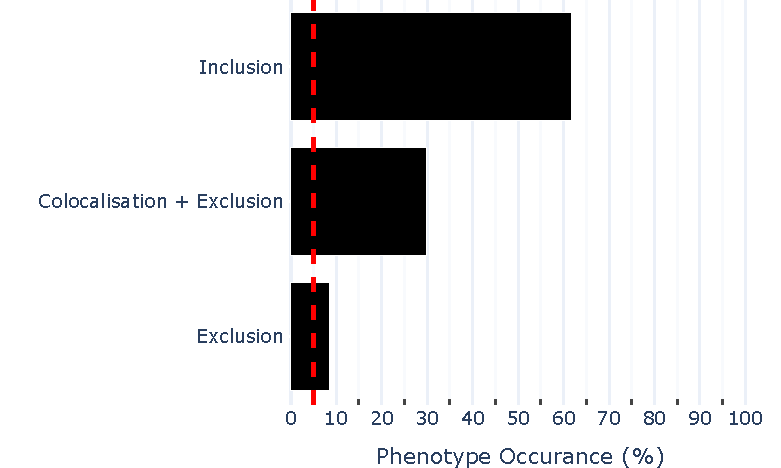
\includegraphics[width=1\linewidth]{08. Chapter 3/Figs/02. Infection/02. IFIT2/01. IFIT2A/01. bar_i2a_a549-n.pdf}
    \end{subfigure}
    \begin{subfigure}{0.495\textwidth}
        \caption{}
        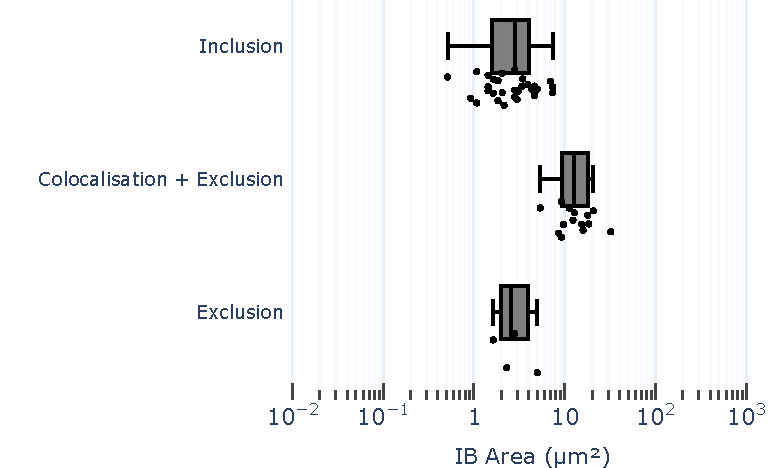
\includegraphics[width=1\linewidth]{08. Chapter 3/Figs/02. Infection/02. IFIT2/01. IFIT2A/02. box_i2a_a549-n.pdf}
    \end{subfigure}
    \caption[Phenotypic Diversity of hIFIT2 Interactions with Nucleoprotein-Stained hRSV Inclusion Bodies, Detected by IFIT2A Antibody in A549 Cell Line.]{\textbf{Phenotypic Diversity of hIFIT2 Interactions with Nucleoprotein-Stained hRSV Inclusion Bodies, Detected by IFIT2A Antibody in A549 Cell Line.} A549 cells were infected with human RSV at MOI 1 and fixed 24 HPI. Cells were labeled with anti-RSV N and anti-IFIT2A antibodies and imaged on confocal microscope. Panel (a) shows percentual proportions of observed phenotypes between hRSV inclusion bodies and hIFIT2, detected by IFIT2A antibody (47 observations), with the red dotted line denoting the 5\% threshold, marking phenotypes considered relevant above this limit. Panel (b) shows the IB area in \(\mu m^2\) per observed relevant phenotype.}
    \label{fig:Phenotypic Diversity of hIFIT2 Interactions with Nucleoprotein-Stained hRSV Inclusion Bodies, Detected by IFIT2A Antibody in A549 Cell Line}
\end{figure}

\begin{figure}
    \centering
    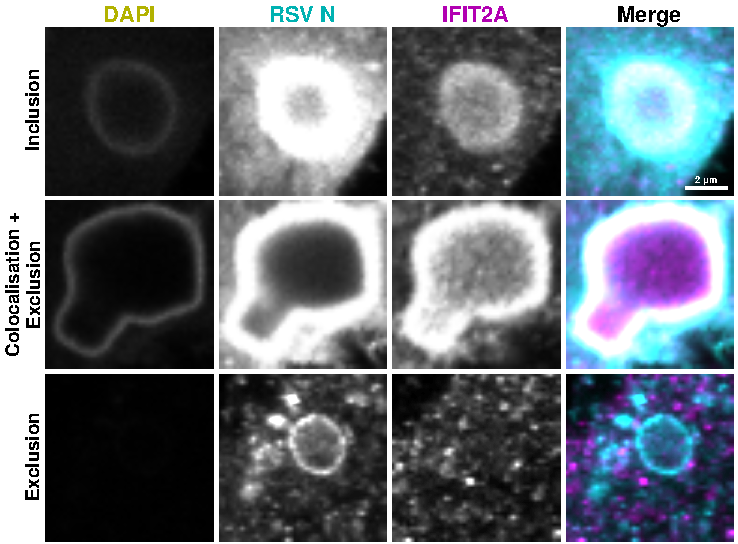
\includegraphics[width=1\linewidth]{08. Chapter 3/Figs/02. Infection/02. IFIT2/01. IFIT2A/03. i2a a549 hrsv n.pdf}
    \caption[Representative Images of Phenotypic Diversity of hIFIT2 Interactions with Nucleoprotein-Stained hRSV Inclusion Bodies, Detected by IFIT2A Antibody in A549 Cell Line.]{\textbf{Representative Images of Phenotypic Diversity of hIFIT2 Interactions with Nucleoprotein-Stained hRSV Inclusion Bodies, Detected by IFIT2A Antibody in A549 Cell Line.} A549 cells were infected with hRSV at MOI 1 and fixed at 24 HPI. Cellular nuclei were stained with DAPI (yellow), and cells were double-labeled with anti-RSV N (cyan) and anti-IFIT2A (magenta) antibodies. This figure showcases representative examples of relevant phenotypes in the interaction between hIFIT2, detected by IFIT2A antibody, and hRSV inclusion bodies. These phenotypes are presented in descending order based on their percentage proportions. The scale bar indicates 2 \(\mu m\).}
    \label{fig:Representative Images of Phenotypic Diversity of hIFIT2 Interactions with Nucleoprotein-Stained hRSV Inclusion Bodies, Detected by IFIT2A Antibody in A549 Cell Line}
\end{figure}

60 30 8

3 12 2.6

Nascent human IFIT2 colocalises with the ring structure (outlined by RSV P staining) and to the inner edge of the IB.

\begin{figure}
    \begin{subfigure}{0.495\textwidth}
        \caption{}
        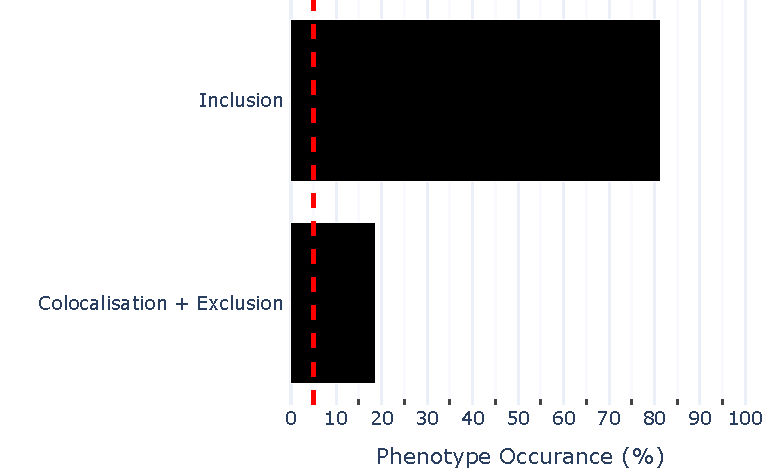
\includegraphics[width=1\linewidth]{08. Chapter 3/Figs/02. Infection/02. IFIT2/01. IFIT2A/04. bar_i2a_a549-p.pdf} 
    \end{subfigure}
    \begin{subfigure}{0.495\textwidth}
        \caption{}
        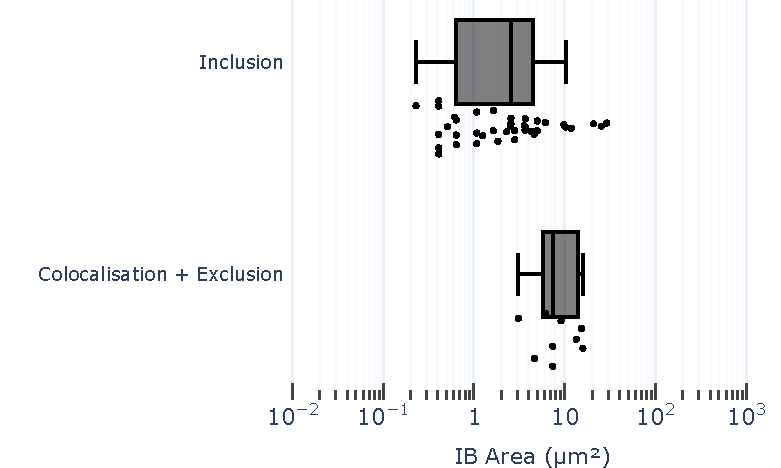
\includegraphics[width=1\linewidth]{08. Chapter 3/Figs/02. Infection/02. IFIT2/01. IFIT2A/05. box_i2a_a549-p.pdf}
    \end{subfigure}
    \caption[Phenotypic Diversity of hIFIT2 Interactions with Phosphoprotein-Stained hRSV Inclusion Bodies, Detected by IFIT2A Antibody in A549 Cell Line.]{\textbf{Phenotypic Diversity of hIFIT2 Interactions with Phosphoprotein-Stained hRSV Inclusion Bodies, Detected by IFIT2A Antibody in A549 Cell Line.} A549 cells were infected with human RSV at MOI 1 and fixed 24 HPI. Cells were labeled with anti-RSV P and anti-IFIT2A antibodies and imaged on confocal microscope. Panel (a) shows percentual proportions of observed phenotypes between hRSV inclusion bodies and hIFIT2, detected by IFIT2A antibody (48 observations), with the red dotted line denoting the 5\% threshold, marking phenotypes considered relevant above this limit. Panel (b) shows the IB area in \(\mu m^2\) per observed relevant phenotype.}
    \label{fig:Phenotypic Diversity of hIFIT2 Interactions with Phosphoprotein-Stained hRSV Inclusion Bodies, Detected by IFIT2A Antibody in A549 Cell Line}
\end{figure}

\begin{figure}
    \centering
    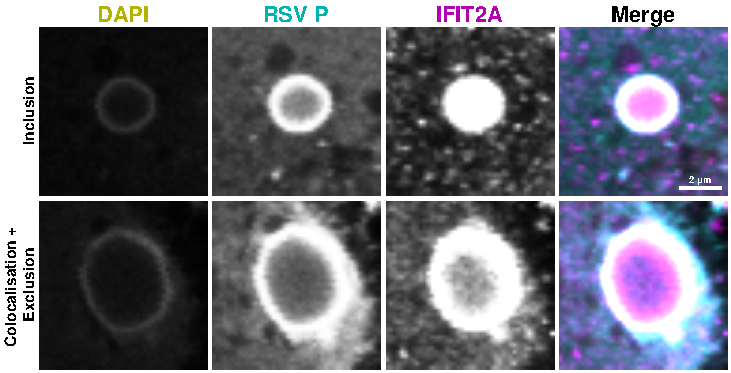
\includegraphics[width=1\linewidth]{08. Chapter 3/Figs/02. Infection/02. IFIT2/01. IFIT2A/06. i2a a549 hrsv p.pdf} 
    \caption[Representative Images of Phenotypic Diversity of hIFIT2 Interactions with Phosphoprotein-Stained hRSV Inclusion Bodies, Detected by IFIT2A Antibody in A549 Cell Line.]{\textbf{Representative Images of Phenotypic Diversity of hIFIT2 Interactions with Phosphoprotein-Stained hRSV Inclusion Bodies, Detected by IFIT2A Antibody in A549 Cell Line.} A549 cells were infected with hRSV at MOI 1 and fixed at 24 HPI. Cellular nuclei were stained with DAPI (yellow), and cells were double-labeled with anti-RSV P (cyan) and anti-IFIT2A (magenta) antibodies. This figure showcases representative examples of relevant phenotypes in the interaction between hIFIT2, detected by IFIT2A antibody, and hRSV inclusion bodies. These phenotypes are presented in descending order based on their percentage proportions. The scale bar indicates 2 \(\mu m\).}
    \label{fig:Representative Images of Phenotypic Diversity of hIFIT2 Interactions with Phosphoprotein-Stained hRSV Inclusion Bodies, Detected by IFIT2A Antibody in A549 Cell Line}
\end{figure}

82 18

2.5 7.3

With regards of colocalization with human RSV M2/1 protein, human IFIT2 seems to either form inclusion, which has a signal decrease towards the middle of the IB structure (top panel), or seems to strongly colocalise with the ring structure highlighted by M2/1 staining (bottom 2 panels; there also seems to be IFIT2 signal concentration on the inner edge of the IB structure).

\begin{figure}
    \begin{subfigure}{0.495\textwidth}
        \caption{}
        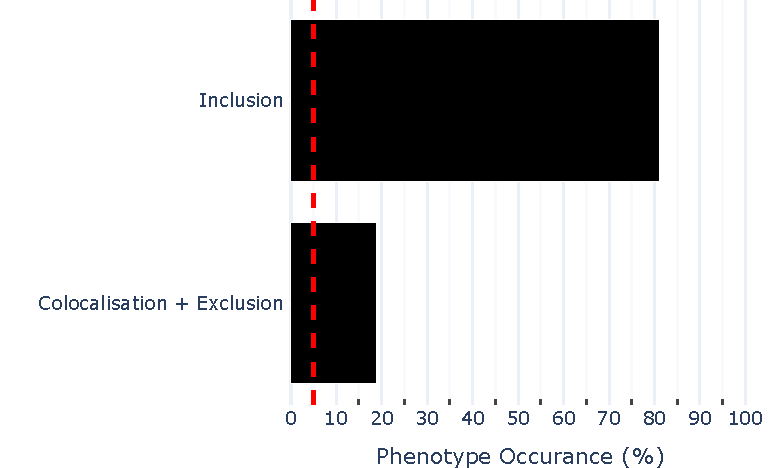
\includegraphics[width=1\linewidth]{08. Chapter 3/Figs/02. Infection/02. IFIT2/01. IFIT2A/07. bar_i2a_a549-m21.pdf} 
    \end{subfigure}
    \begin{subfigure}{0.495\textwidth}
        \caption{}
        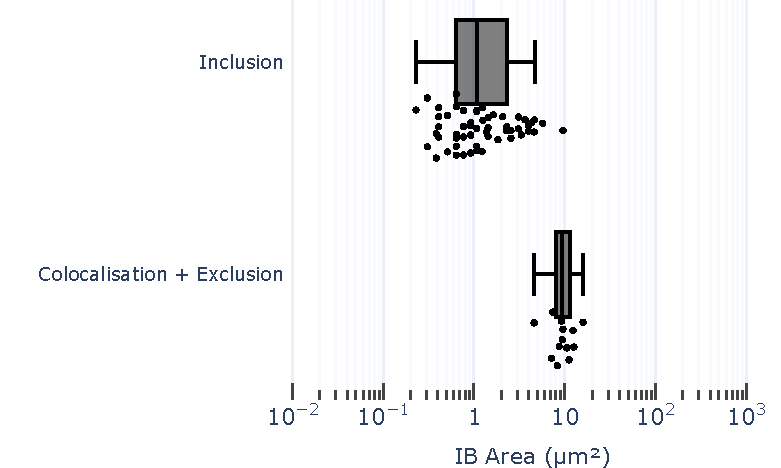
\includegraphics[width=1\linewidth]{08. Chapter 3/Figs/02. Infection/02. IFIT2/01. IFIT2A/08. box_i2a_a549-m21.pdf}
    \end{subfigure}
    \caption[Phenotypic Diversity of hIFIT2 Interactions with M2/1-Stained hRSV Inclusion Bodies, Detected by IFIT2A Antibody in A549 Cell Line.]{\textbf{Phenotypic Diversity of hIFIT2 Interactions with M2/1-Stained hRSV Inclusion Bodies, Detected by IFIT2A Antibody in A549 Cell Line.} A549 cells were infected with human RSV at MOI 1 and fixed 24 HPI. Cells were labeled with anti-RSV M2/1 and anti-IFIT2A antibodies and imaged on confocal microscope. Panel (a) shows percentual proportions of observed phenotypes between hRSV inclusion bodies and hIFIT2, detected by IFIT2A antibody (69 observations), with the red dotted line denoting the 5\% threshold, marking phenotypes considered relevant above this limit. Panel (b) shows the IB area in \(\mu m^2\) per observed relevant phenotype.}
    \label{fig:Phenotypic Diversity of hIFIT2 Interactions with M2/1-Stained hRSV Inclusion Bodies, Detected by IFIT2A Antibody in A549 Cell Line}
\end{figure}

\begin{figure}
    \centering
    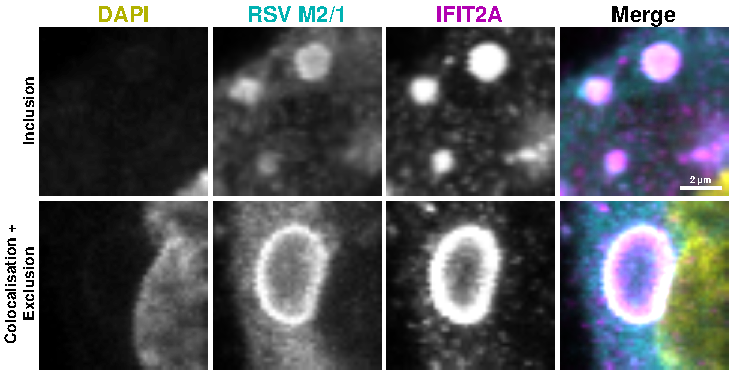
\includegraphics[width=1\linewidth]{08. Chapter 3/Figs/02. Infection/02. IFIT2/01. IFIT2A/09. i2a a549 hrsv m21.pdf} 
    \caption[Representative Images of Phenotypic Diversity of hIFIT2 Interactions with M2/1-Stained hRSV Inclusion Bodies, Detected by IFIT2A Antibody in A549 Cell Line.]{\textbf{Representative Images of Phenotypic Diversity of hIFIT2 Interactions with M2/1-Stained hRSV Inclusion Bodies, Detected by IFIT2A Antibody in A549 Cell Line.} A549 cells were infected with hRSV at MOI 1 and fixed at 24 HPI. Cellular nuclei were stained with DAPI (yellow), and cells were double-labeled with anti-RSV M2/1 (cyan) and anti-IFIT2A (magenta) antibodies. This figure showcases representative examples of relevant phenotypes in the interaction between hIFIT2, detected by IFIT2A antibody, and hRSV inclusion bodies. These phenotypes are presented in descending order based on their percentage proportions. The scale bar indicates 2 \(\mu m\).}
    \label{fig:Representative Images of Phenotypic Diversity of hIFIT2 Interactions with M2/1-Stained hRSV Inclusion Bodies, Detected by IFIT2A Antibody in A549 Cell Line}
\end{figure}

81 19

1 10

\begin{figure}
    \begin{subfigure}{0.495\textwidth}
        \caption{}
        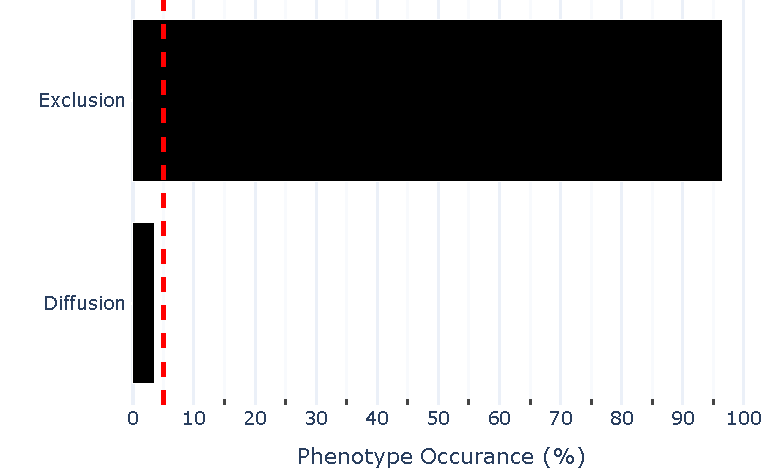
\includegraphics[width=1\linewidth]{08. Chapter 3/Figs/02. Infection/02. IFIT2/02. IFIT2B/01. bar_i2b_a549-n.pdf}
    \end{subfigure}
    \begin{subfigure}{0.495\textwidth}
        \caption{}
        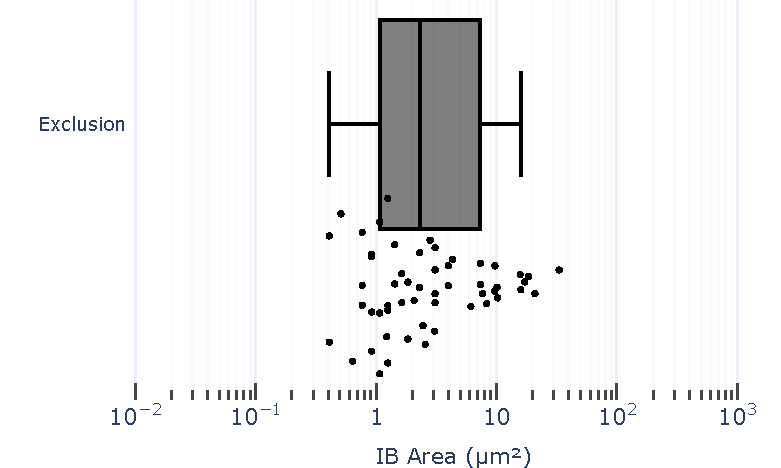
\includegraphics[width=1\linewidth]{08. Chapter 3/Figs/02. Infection/02. IFIT2/02. IFIT2B/02. box_i2b_a549-n.pdf}
    \end{subfigure}
    \caption[Phenotypic Diversity of hIFIT2 Interactions with Nucleoprotein-Stained hRSV Inclusion Bodies, Detected by IFIT2B Antibody in A549 Cell Line.]{\textbf{Phenotypic Diversity of hIFIT2 Interactions with Nucleoprotein-Stained hRSV Inclusion Bodies, Detected by IFIT2B Antibody in A549 Cell Line.} A549 cells were infected with human RSV at MOI 1 and fixed 24 HPI. Cells were labeled with anti-RSV N and anti-IFIT2B antibodies and imaged on confocal microscope. Panel (a) shows percentual proportions of observed phenotypes between hRSV inclusion bodies and hIFIT2, detected by IFIT2B antibody (56 observations), with the red dotted line denoting the 5\% threshold, marking phenotypes considered relevant above this limit. Panel (b) shows the IB area in \(\mu m^2\) per observed relevant phenotype.}
    \label{fig:Phenotypic Diversity of hIFIT2 Interactions with Nucleoprotein-Stained hRSV Inclusion Bodies, Detected by IFIT2B Antibody in A549 Cell Line}
\end{figure}

\begin{figure}
    \centering
    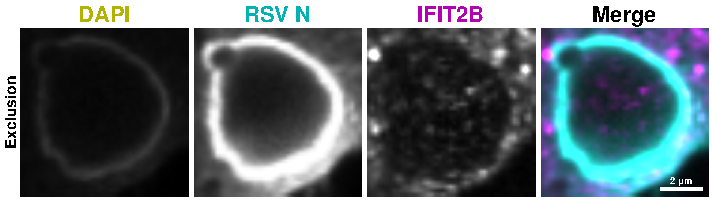
\includegraphics[width=1\linewidth]{08. Chapter 3/Figs/02. Infection/02. IFIT2/02. IFIT2B/03. i2b a549 hrsv n.pdf} 
    \caption[Representative Images of Phenotypic Diversity of hIFIT2 Interactions with Nucleoprotein-Stained hRSV Inclusion Bodies, Detected by IFIT2B Antibody in A549 Cell Line.]{\textbf{Representative Images of Phenotypic Diversity of hIFIT2 Interactions with Nucleoprotein-Stained hRSV Inclusion Bodies, Detected by IFIT2B Antibody in A549 Cell Line.} A549 cells were infected with hRSV at MOI 1 and fixed at 24 HPI. Cellular nuclei were stained with DAPI (yellow), and cells were double-labeled with anti-RSV N (cyan) and anti-IFIT2B (magenta) antibodies. This figure showcases representative examples of relevant phenotypes in the interaction between hIFIT2, detected by IFIT2B antibody, and hRSV inclusion bodies. These phenotypes are presented in descending order based on their percentage proportions. The scale bar indicates 2 \(\mu m\).}
    \label{fig:Representative Images of Phenotypic Diversity of hIFIT2 Interactions with Nucleoprotein-Stained hRSV Inclusion Bodies, Detected by IFIT2B Antibody in A549 Cell Line}
\end{figure}

96

2.1

Endogenous human IFIT2 is either partially excluded (top panel; decrease of intra IB signal compared to cytoplasmic signal) or completely excluded (bottom panel) from the human IB structure.

\begin{figure}
    \begin{subfigure}{0.495\textwidth}
        \caption{}
        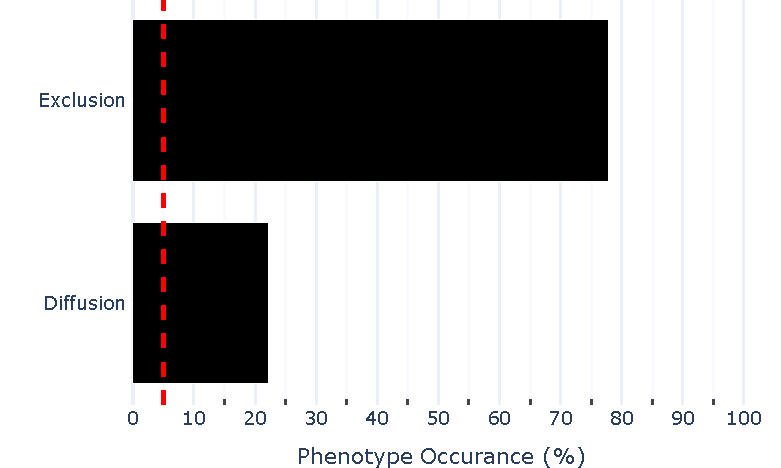
\includegraphics[width=1\linewidth]{08. Chapter 3/Figs/02. Infection/02. IFIT2/02. IFIT2B/04. bar_i2b_a549-p.pdf} 
    \end{subfigure}
    \begin{subfigure}{0.495\textwidth}
        \caption{}
        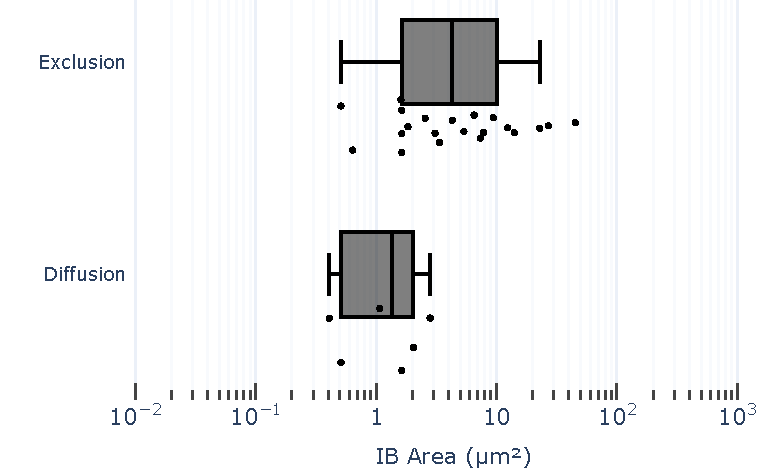
\includegraphics[width=1\linewidth]{08. Chapter 3/Figs/02. Infection/02. IFIT2/02. IFIT2B/05. box_i2b_a549-p.pdf}
    \end{subfigure}
    \caption[Phenotypic Diversity of hIFIT2 Interactions with Phosphoprotein-Stained hRSV Inclusion Bodies, Detected by IFIT2B Antibody in A549 Cell Line.]{\textbf{Phenotypic Diversity of hIFIT2 Interactions with Phosphoprotein-Stained hRSV Inclusion Bodies, Detected by IFIT2B Antibody in A549 Cell Line.} A549 cells were infected with human RSV at MOI 1 and fixed 24 HPI. Cells were labeled with anti-RSV P and anti-IFIT2B antibodies and imaged on confocal microscope. Panel (a) shows percentual proportions of observed phenotypes between hRSV inclusion bodies and hIFIT2, detected by IFIT2B antibody (27 observations), with the red dotted line denoting the 5\% threshold, marking phenotypes considered relevant above this limit. Panel (b) shows the IB area in \(\mu m^2\) per observed relevant phenotype.}
    \label{fig:Phenotypic Diversity of hIFIT2 Interactions with Phosphoprotein-Stained hRSV Inclusion Bodies, Detected by IFIT2B Antibody in A549 Cell Line}
\end{figure}

\begin{figure}
    \centering
    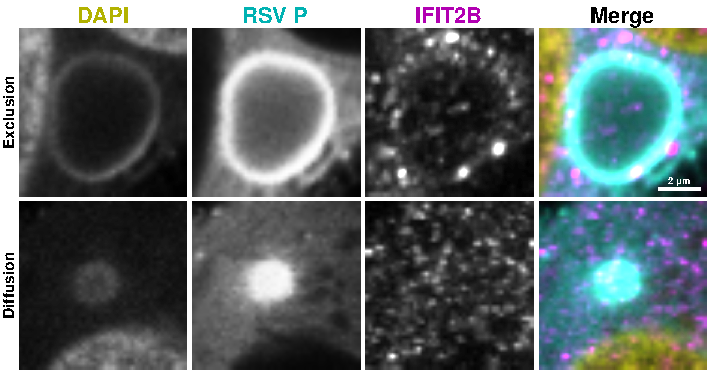
\includegraphics[width=1\linewidth]{08. Chapter 3/Figs/02. Infection/02. IFIT2/02. IFIT2B/06. i2b a549 hrsv p.pdf} 
    \caption[Representative Images of Phenotypic Diversity of hIFIT2 Interactions with Phosphoprotein-Stained hRSV Inclusion Bodies, Detected by IFIT2B Antibody in A549 Cell Line.]{\textbf{Representative Images of Phenotypic Diversity of hIFIT2 Interactions with Phosphoprotein-Stained hRSV Inclusion Bodies, Detected by IFIT2B Antibody in A549 Cell Line.} A549 cells were infected with hRSV at MOI 1 and fixed at 24 HPI. Cellular nuclei were stained with DAPI (yellow), and cells were double-labeled with anti-RSV P (cyan) and anti-IFIT2B (magenta) antibodies. This figure showcases representative examples of relevant phenotypes in the interaction between hIFIT2, detected by IFIT2B antibody, and hRSV inclusion bodies. These phenotypes are presented in descending order based on their percentage proportions. The scale bar indicates 2 \(\mu m\).}
    \label{fig:Representative Images of Phenotypic Diversity of hIFIT2 Interactions with Phosphoprotein-Stained hRSV Inclusion Bodies, Detected by IFIT2B Antibody in A549 Cell Line}
\end{figure}

78 22

4.3 1.3

We observe similar pattern of staining to what was observed with N stained human IBs. IFIT2 signal is either partially or totally excluded from the IB structure.

\begin{figure}
    \begin{subfigure}{0.495\textwidth}
        \caption{}
        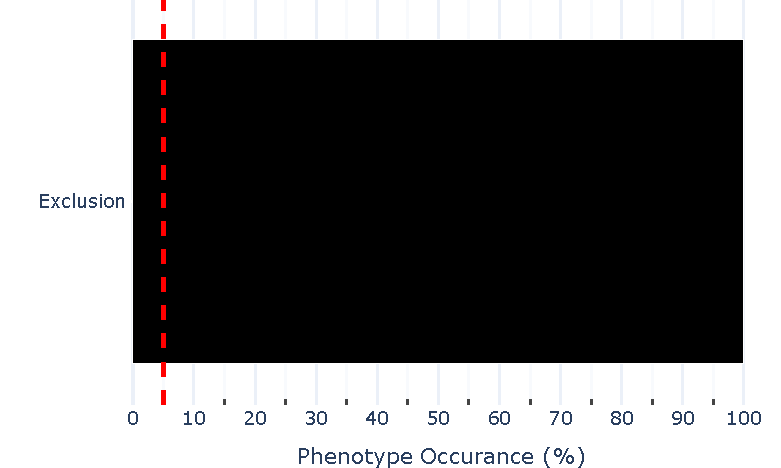
\includegraphics[width=1\linewidth]{08. Chapter 3/Figs/02. Infection/02. IFIT2/02. IFIT2B/07. bar_i2b_a549-m21.pdf} 
    \end{subfigure}
    \begin{subfigure}{0.495\textwidth}
        \caption{}
        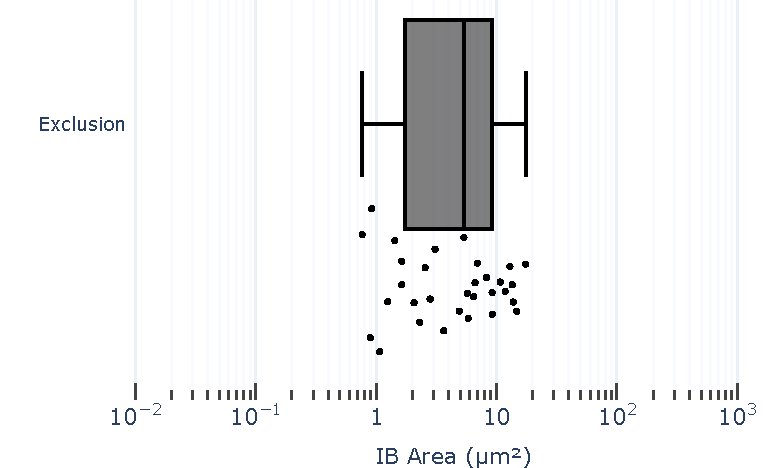
\includegraphics[width=1\linewidth]{08. Chapter 3/Figs/02. Infection/02. IFIT2/02. IFIT2B/08. box_i2b_a549-m21.pdf}
    \end{subfigure}
    \caption[Phenotypic Diversity of hIFIT2 Interactions with M2/1-Stained hRSV Inclusion Bodies, Detected by IFIT2B Antibody in A549 Cell Line.]{\textbf{Phenotypic Diversity of hIFIT2 Interactions with M2/1-Stained hRSV Inclusion Bodies, Detected by IFIT2B Antibody in A549 Cell Line.} A549 cells were infected with human RSV at MOI 1 and fixed 24 HPI. Cells were labeled with anti-RSV M2/1 and anti-IFIT2B antibodies and imaged on confocal microscope. Panel (a) shows percentual proportions of observed phenotypes between hRSV inclusion bodies and hIFIT2, detected by IFIT2B antibody (31 observations), with the red dotted line denoting the 5\% threshold, marking phenotypes considered relevant above this limit. Panel (b) shows the IB area in \(\mu m^2\) per observed relevant phenotype.}
    \label{fig:Phenotypic Diversity of hIFIT2 Interactions with M2/1-Stained hRSV Inclusion Bodies, Detected by IFIT2B Antibody in A549 Cell Line}
\end{figure}

\begin{figure}
    \centering
    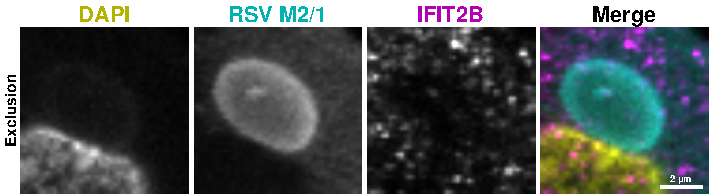
\includegraphics[width=1\linewidth]{08. Chapter 3/Figs/02. Infection/02. IFIT2/02. IFIT2B/09. i2b a549 hrsv m21.pdf} 
    \caption[Representative Images of Phenotypic Diversity of hIFIT2 Interactions with M2/1-Stained hRSV Inclusion Bodies, Detected by IFIT2B Antibody in A549 Cell Line.]{\textbf{Representative Images of Phenotypic Diversity of hIFIT2 Interactions with M2/1-Stained hRSV Inclusion Bodies, Detected by IFIT2B Antibody in A549 Cell Line.} A549 cells were infected with hRSV at MOI 1 and fixed at 24 HPI. Cellular nuclei were stained with DAPI (yellow), and cells were double-labeled with anti-RSV M2/1 (cyan) and anti-IFIT2B (magenta) antibodies. This figure showcases representative examples of relevant phenotypes in the interaction between hIFIT2, detected by IFIT2B antibody, and hRSV inclusion bodies. These phenotypes are presented in descending order based on their percentage proportions. The scale bar indicates 2 \(\mu m\).}
    \label{fig:Representative Images of Phenotypic Diversity of hIFIT2 Interactions with M2/1-Stained hRSV Inclusion Bodies, Detected by IFIT2B Antibody in A549 Cell Line}
\end{figure}

71 21 6

2.1 8 15

Endogenous human IFIT2 seems to be excluded from hRSV IBs.

\begin{figure}
    \begin{subfigure}{0.495\textwidth}
        \caption{}
        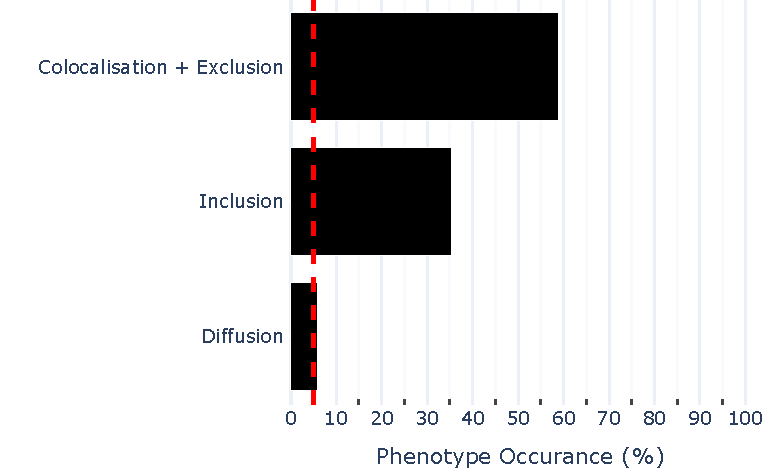
\includegraphics[width=1\linewidth]{08. Chapter 3/Figs/02. Infection/02. IFIT2/01. IFIT2A/10. bar_i2a_beas2b.pdf} 
    \end{subfigure}
    \begin{subfigure}{0.495\textwidth}
        \caption{}
        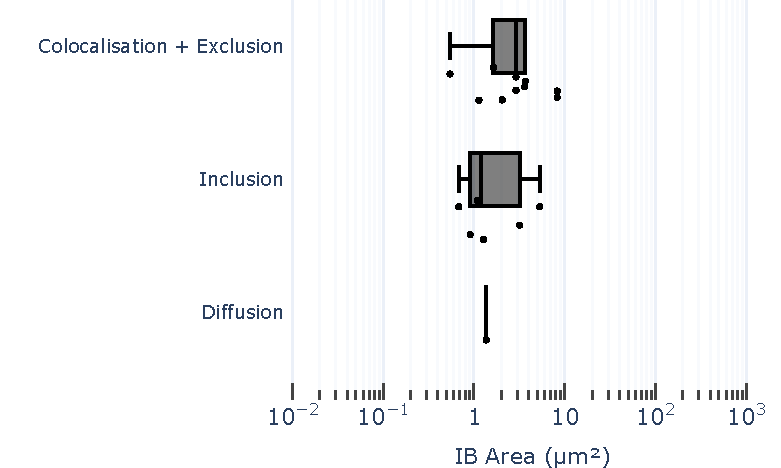
\includegraphics[width=1\linewidth]{08. Chapter 3/Figs/02. Infection/02. IFIT2/01. IFIT2A/11. box_i2a_beas2b.pdf}
    \end{subfigure}
    \caption[Phenotypic Diversity of hIFIT2 Interactions with hRSV Inclusion Bodies, Detected by IFIT2A Antibody in BEAS2B Cell Line.]{\textbf{Phenotypic Diversity of hIFIT2 Interactions with hRSV Inclusion Bodies, Detected by IFIT2A Antibody in BEAS2B Cell Line.} BEAS2B cells were infected with human RSV at MOI 1 and fixed 24 HPI. Cells were labeled with anti-RSV N and anti-IFIT2A antibodies and imaged on confocal microscope. Panel (a) shows percentual proportions of observed phenotypes between hRSV inclusion bodies and hIFIT2, detected by IFIT2A antibody (99 observations), with the red dotted line denoting the 5\% threshold, marking phenotypes considered relevant above this limit. Panel (b) shows the IB area in \(\mu m^2\) per observed relevant phenotype.}
    \label{fig:Phenotypic Diversity of hIFIT2 Interactions with hRSV Inclusion Bodies, Detected by IFIT2A Antibody in BEAS2B Cell Line}
\end{figure}

\begin{figure}
    \centering
    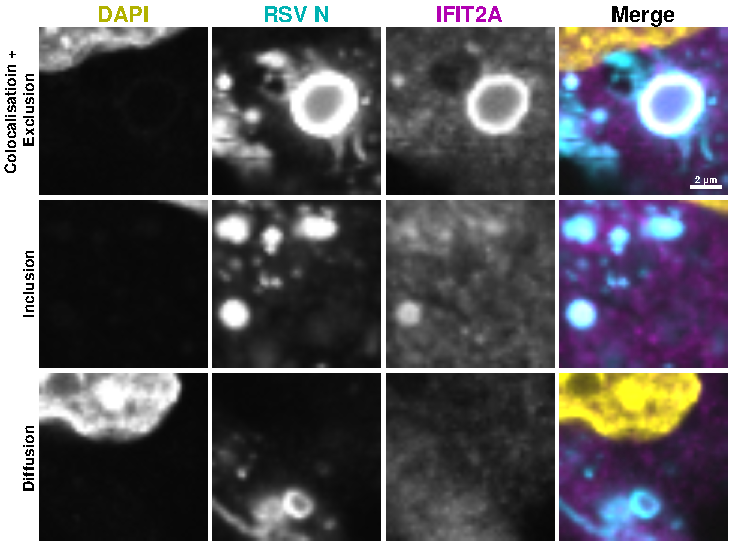
\includegraphics[width=1\linewidth]{08. Chapter 3/Figs/02. Infection/02. IFIT2/01. IFIT2A/12. i2a beas2b.pdf} 
    \caption[Representative Images of Phenotypic Diversity of hIFIT2 Interactions with hRSV Inclusion Bodies, Detected by IFIT2A Antibody in BEAS2B Cell Line.]{\textbf{Representative Images of Phenotypic Diversity of hIFIT2 Interactions with hRSV Inclusion Bodies, Detected by IFIT2A Antibody in BEAS2B Cell Line.} BEAS2B cells were infected with hRSV at MOI 1 and fixed at 24 HPI. Cellular nuclei were stained with DAPI (yellow), and cells were double-labeled with anti-RSV N (cyan) and anti-IFIT2A (magenta) antibodies. This figure showcases representative examples of relevant phenotypes in the interaction between hIFIT2, detected by IFIT2A antibody, and hRSV inclusion bodies. These phenotypes are presented in descending order based on their percentage proportions. The scale bar indicates 2 \(\mu m\).}
    \label{fig:Representative Images of Phenotypic Diversity of hIFIT2 Interactions with hRSV Inclusion Bodies, Detected by IFIT2A Antibody in BEAS2B Cell Line}
\end{figure}

58 35 5

3 1.2 1.2


Nascent bovine IFIT2 colocalization with regards of N stained bRSV IBs seems to strongly associate with the ring of the structure.

\begin{figure}
    \begin{subfigure}{0.495\textwidth}
        \caption{}
        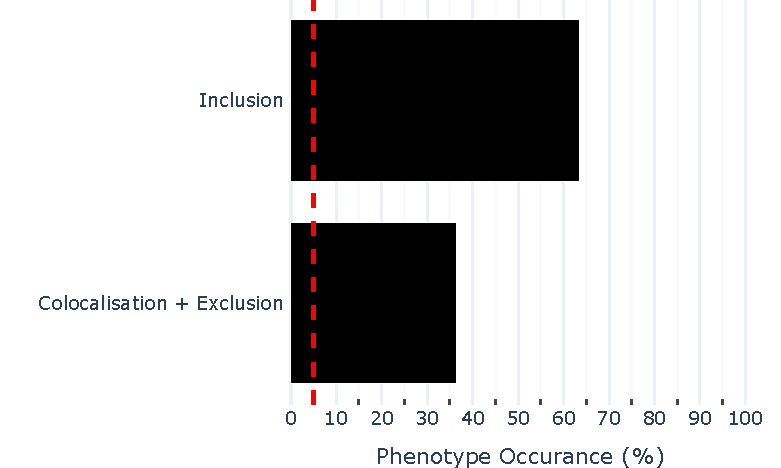
\includegraphics[width=1\linewidth]{08. Chapter 3/Figs/02. Infection/02. IFIT2/01. IFIT2A/13. bar_i2a_mdbk.pdf} 
    \end{subfigure}
    \begin{subfigure}{0.495\textwidth}
        \caption{}
        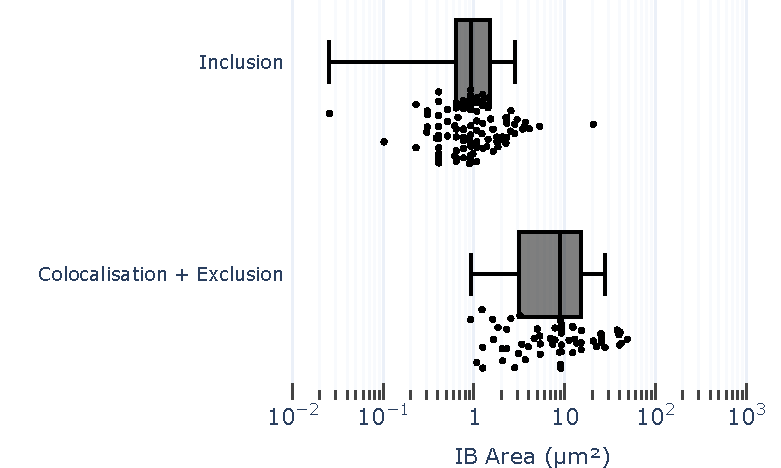
\includegraphics[width=1\linewidth]{08. Chapter 3/Figs/02. Infection/02. IFIT2/01. IFIT2A/14. box_i2a_mdbk.pdf}
    \end{subfigure}
    \caption[Phenotypic Diversity of hIFIT2 Interactions with bRSV Inclusion Bodies, Detected by IFIT2A Antibody in MDBK Cell Line.]{\textbf{Phenotypic Diversity of hIFIT2 Interactions with bRSV Inclusion Bodies, Detected by IFIT2A Antibody in MDBK Cell Line.} MDBK cells were infected with bovine RSV at MOI 1 and fixed 24 HPI. Cells were labeled with anti-RSV N and anti-IFIT2A antibodies and imaged on confocal microscope. Panel (a) shows percentual proportions of observed phenotypes between bRSV inclusion bodies and bIFIT2, detected by IFIT2A antibody (162 observations), with the red dotted line denoting the 5\% threshold, marking phenotypes considered relevant above this limit. Panel (b) shows the IB area in \(\mu m^2\) per observed relevant phenotype.}
    \label{fig:Phenotypic Diversity of hIFIT2 Interactions with bRSV Inclusion Bodies, Detected by IFIT2A Antibody in MDBK Cell Line}
\end{figure}

\begin{figure}
    \centering
    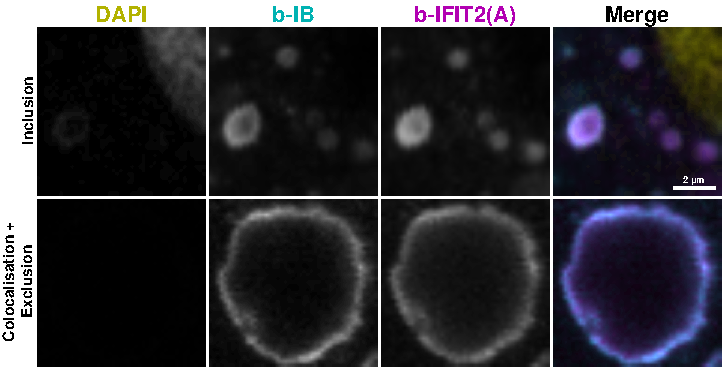
\includegraphics[width=1\linewidth]{08. Chapter 3/Figs/02. Infection/02. IFIT2/01. IFIT2A/15. i2a mdbk brsv.pdf} 
    \caption[Representative Images of Phenotypic Diversity of hIFIT2 Interactions with bRSV Inclusion Bodies, Detected by IFIT2A Antibody in MDBK Cell Line.]{\textbf{Representative Images of Phenotypic Diversity of hIFIT2 Interactions with bRSV Inclusion Bodies, Detected by IFIT2A Antibody in MDBK Cell Line.} MDBK cells were infected with bRSV at MOI 1 and fixed at 24 HPI. Cellular nuclei were stained with DAPI (yellow), and cells were double-labeled with anti-RSV N (cyan) and anti-IFIT2A (magenta) antibodies. This figure showcases representative examples of relevant phenotypes in the interaction between bIFIT2, detected by IFIT2A antibody, and bRSV inclusion bodies. These phenotypes are presented in descending order based on their percentage proportions. The scale bar indicates 2 \(\mu m\).}
    \label{fig:Representative Images of Phenotypic Diversity of hIFIT2 Interactions with bRSV Inclusion Bodies, Detected by IFIT2A Antibody in MDBK Cell Line}
\end{figure}

64 36

1 9

\begin{figure}
    \begin{subfigure}{0.495\textwidth}
        \caption{}
        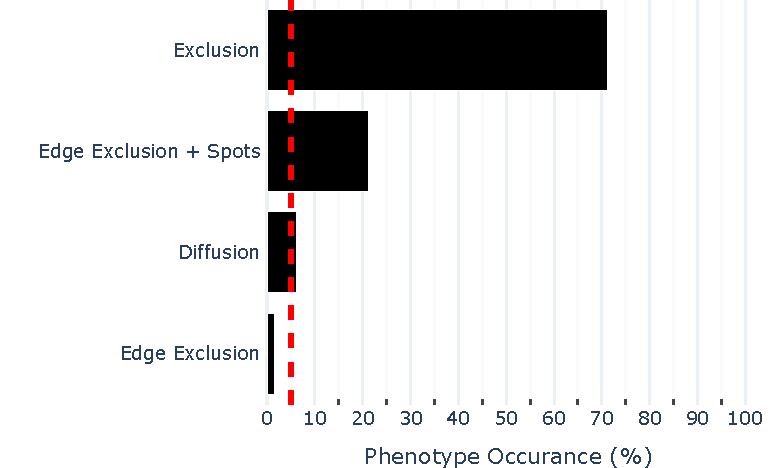
\includegraphics[width=1\linewidth]{08. Chapter 3/Figs/02. Infection/02. IFIT2/02. IFIT2B/10. bar_i2b_mdbk.pdf} 
    \end{subfigure}
    \begin{subfigure}{0.495\textwidth}
        \caption{}
        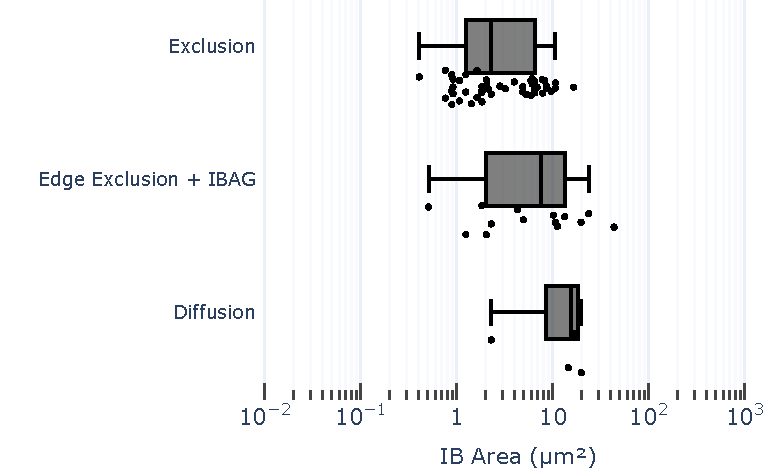
\includegraphics[width=1\linewidth]{08. Chapter 3/Figs/02. Infection/02. IFIT2/02. IFIT2B/11. box_i2b_mdbk.pdf}
    \end{subfigure}
    \caption[Phenotypic Diversity of hIFIT2 Interactions with bRSV Inclusion Bodies, Detected by IFIT2B Antibody in MDBK Cell Line.]{\textbf{Phenotypic Diversity of hIFIT2 Interactions with bRSV Inclusion Bodies, Detected by IFIT2B Antibody in MDBK Cell Line.} MDBK cells were infected with bovine RSV at MOI 1 and fixed 24 HPI. Cells were labeled with anti-RSV N and anti-IFIT2B antibodies and imaged on confocal microscope. Panel (a) shows percentual proportions of observed phenotypes between bRSV inclusion bodies and bIFIT2, detected by IFIT2B antibody (66 observations), with the red dotted line denoting the 5\% threshold, marking phenotypes considered relevant above this limit. Panel (b) shows the IB area in \(\mu m^2\) per observed relevant phenotype.}
    \label{fig:Phenotypic Diversity of hIFIT2 Interactions with bRSV Inclusion Bodies, Detected by IFIT2B Antibody in MDBK Cell Line}
\end{figure}

\begin{figure}
    \centering
    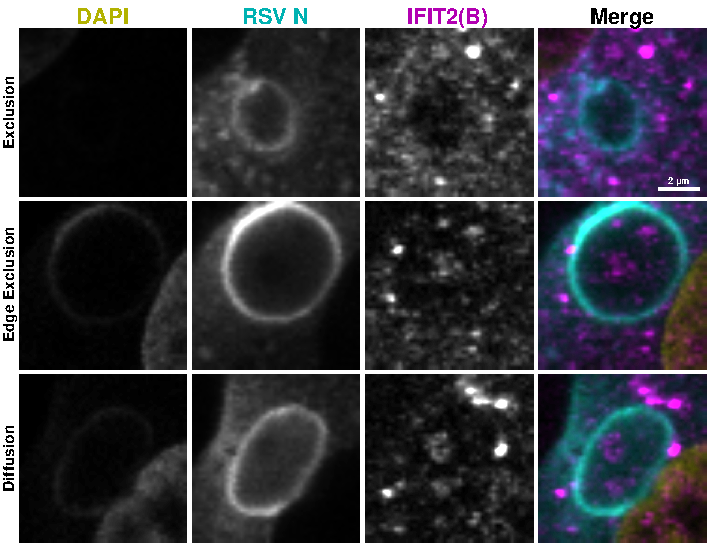
\includegraphics[width=1\linewidth]{08. Chapter 3/Figs/02. Infection/02. IFIT2/02. IFIT2B/12. i2b mdbk brsv.pdf} 
    \caption[Representative Images of Phenotypic Diversity of hIFIT2 Interactions with bRSV Inclusion Bodies, Detected by IFIT2B Antibody in MDBK Cell Line.]{\textbf{Representative Images of Phenotypic Diversity of hIFIT2 Interactions with bRSV Inclusion Bodies, Detected by IFIT2B Antibody in MDBK Cell Line.} MDBK cells were infected with bRSV at MOI 1 and fixed at 24 HPI. Cellular nuclei were stained with DAPI (yellow), and cells were double-labeled with anti-RSV N (cyan) and anti-IFIT2B (magenta) antibodies. This figure showcases representative examples of relevant phenotypes in the interaction between bIFIT2, detected by IFIT2B antibody, and bRSV inclusion bodies. These phenotypes are presented in descending order based on their percentage proportions. The scale bar indicates 2 \(\mu m\).}
    \label{fig:Representative Images of Phenotypic Diversity of hIFIT2 Interactions with bRSV Inclusion Bodies, Detected by IFIT2B Antibody in MDBK Cell Line}
\end{figure}

71 21 6

2 8 17

\subsubsection{Phenotypic Diversity of Nascent IFIT3 Interaction with RSV Inclusion Bodies}
Nascent human IFIT3 seems to have mainly diffused phenotype (top and bottom panel) with occasional exclusion without any marked IFIT3 concentration adjacent to the IB structure (middle panel).

53, 17, 16, 10

4.5, 12, 5, 1.9

\begin{figure}
    \begin{subfigure}{0.495\textwidth}
        \caption{}
        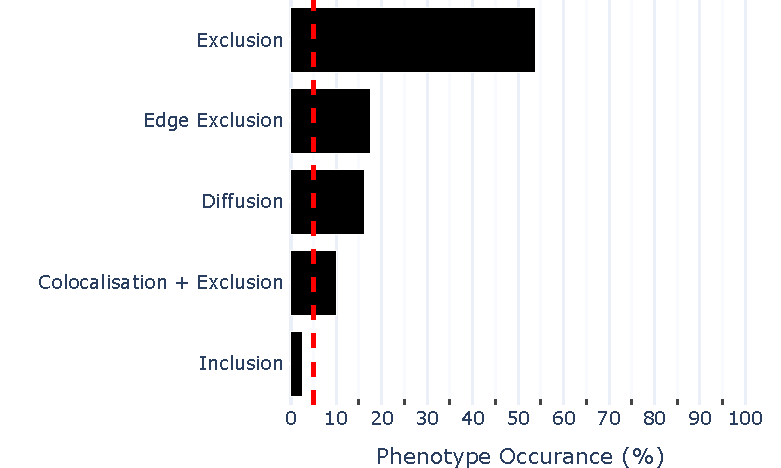
\includegraphics[width=1\linewidth]{08. Chapter 3/Figs/02. Infection/03. IFIT3/01. bar_i3_a549.pdf} 
    \end{subfigure}
    \begin{subfigure}{0.495\textwidth}
        \caption{}
        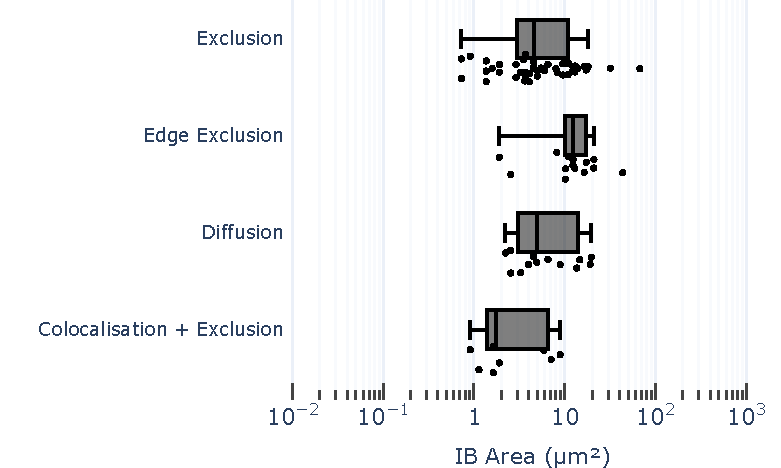
\includegraphics[width=1\linewidth]{08. Chapter 3/Figs/02. Infection/03. IFIT3/02. box_i3_a549.pdf}
    \end{subfigure}
    \caption[Phenotypic Diversity of hIFIT3 Interactions with hRSV Inclusion Bodies in A549 Cell Line.]{\textbf{Phenotypic Diversity of hIFIT3 Interactions with hRSV Inclusion Bodies in A549 Cell Line.} A549 cells were infected with human RSV at MOI 1 and fixed 24 HPI. Cells were double-labeled with with anti-RSV N and anti-IFIT3 antibodies and imaged on confocal microscope. Panel (a) shows percentual proportions of observed phenotypes between hRSV inclusion bodies and hIFIT3 (80 observations), with the red dotted line denoting the 5\% threshold, marking phenotypes considered relevant above this limit. Panel (b) shows the IB area in \(\mu m^2\) per observed relevant phenotype.}
    \label{fig:Phenotypic Diversity of hIFIT3 Interactions with hRSV Inclusion Bodies in A549 Cell Line}
\end{figure}

\begin{figure}
    \centering
    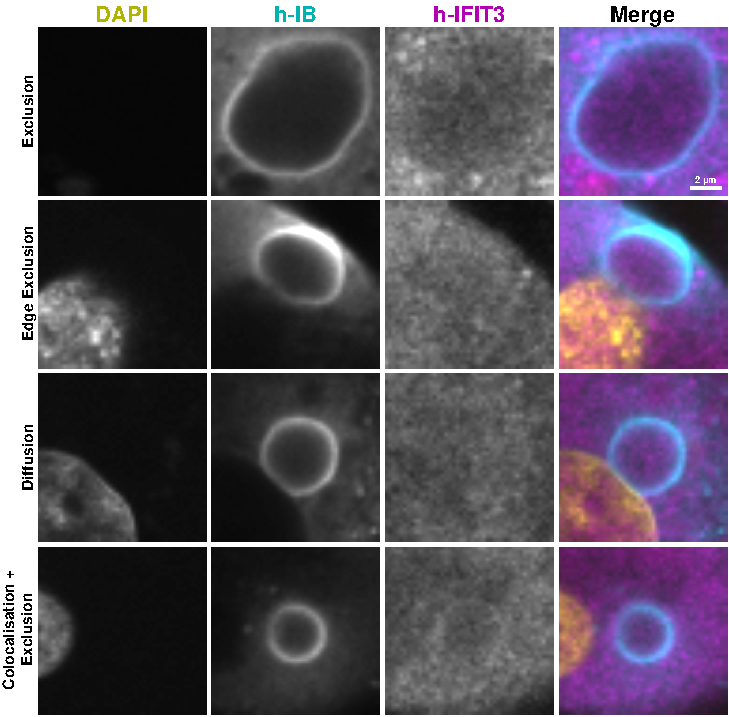
\includegraphics[width=1\linewidth]{08. Chapter 3/Figs/02. Infection/03. IFIT3/03. a549 i3.pdf}
    \caption[Representative Images of Phenotypic Diversity of hIFIT3 Interactions with hRSV Inclusion Bodies in A549 Cell Line.]{\textbf{Representative Images of Phenotypic Diversity of hIFIT3 Interactions with hRSV Inclusion Bodies in A549 Cell Line.} A549 cells were infected with hRSV at MOI 1 and fixed at 24 HPI. Cellular nuclei were stained with DAPI (yellow), and cells were double-labeled with anti-RSV N (cyan) and anti-IFIT3 (magenta) antibodies. This figure showcases representative examples of relevant phenotypes in the interaction between hIFIT3 and hRSV inclusion bodies. These phenotypes are presented in descending order based on their percentage proportions. The scale bar indicates 2 \(\mu m\).}
    \label{fig:Representative Images of Phenotypic Diversity of hIFIT3 Interactions with hRSV Inclusion Bodies in A549 Cell Line}
\end{figure}

62, 19, 12

5.5, 3, 10, 2.3

\begin{figure}
    \begin{subfigure}{0.495\textwidth}
        \caption{}
        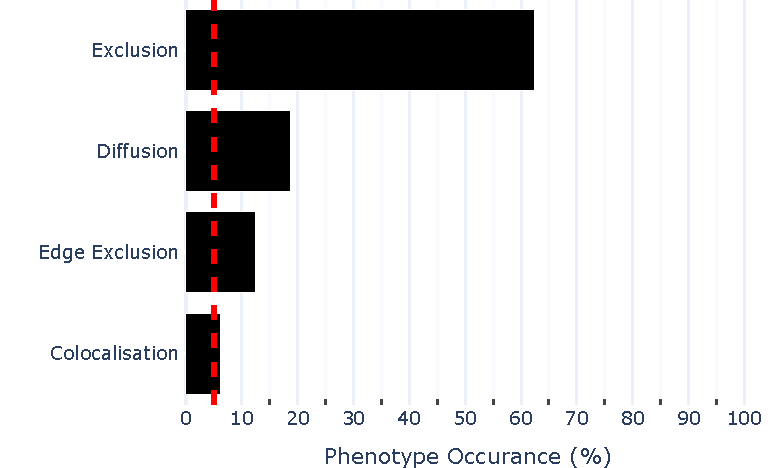
\includegraphics[width=1\linewidth]{08. Chapter 3/Figs/02. Infection/03. IFIT3/04. bar_i3_beas2b.pdf} 
    \end{subfigure}
    \begin{subfigure}{0.495\textwidth}
        \caption{}        
        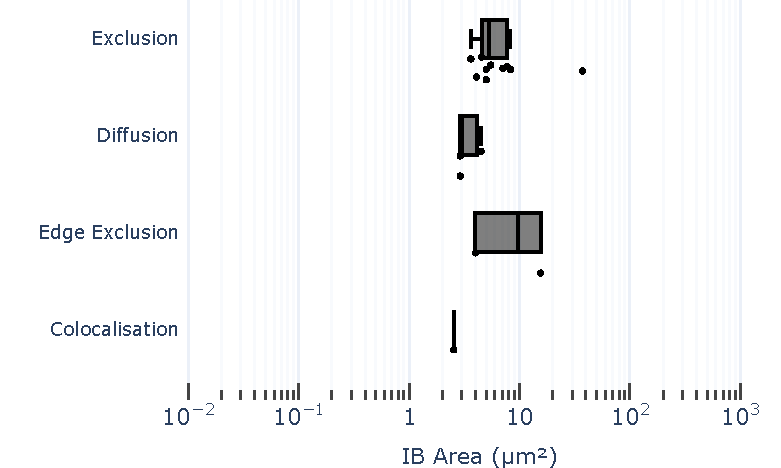
\includegraphics[width=1\linewidth]{08. Chapter 3/Figs/02. Infection/03. IFIT3/05. box_i3_beas2b.pdf}
    \end{subfigure}
    \caption[Phenotypic Diversity of hIFIT3 Interactions with hRSV Inclusion Bodies in BEAS2B Cell Line.]{\textbf{Phenotypic Diversity of hIFIT3 Interactions with hRSV Inclusion Bodies in BEAS2B Cell Line.} BEAS2B cells were infected with human RSV at MOI 1 and fixed 24 HPI. Cells were labeled with anti-RSV N and anti-IFIT3 antibodies and imaged on confocal microscope. Panel (a) shows percentual proportions of observed phenotypes between hRSV inclusion bodies and hIFIT3 (16 observations), with the red dotted line denoting the 5\% threshold, marking phenotypes considered relevant above this limit. Panel (b) shows the IB area in \(\mu m^2\) per observed relevant phenotype.}
    \label{fig:Phenotypic Diversity of hIFIT3 Interactions with hRSV Inclusion Bodies in BEAS2B Cell Line}
\end{figure}

\begin{figure}
    \centering
    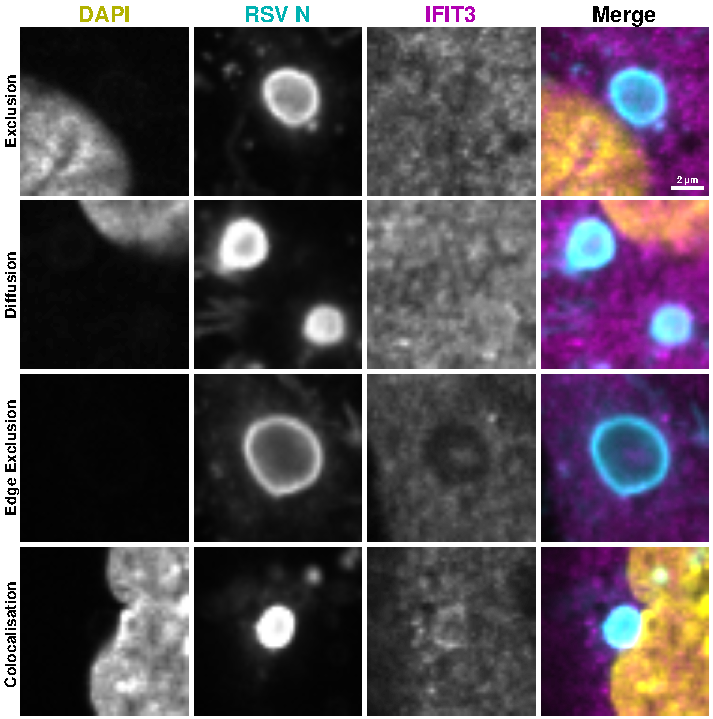
\includegraphics[width=1\linewidth]{08. Chapter 3/Figs/02. Infection/03. IFIT3/06. beas2b i3.pdf}
    \caption[Representative Images of Phenotypic Diversity of hIFIT3 Interactions with hRSV Inclusion Bodies in BEAS2B Cell Line]{\textbf{Representative Images of Phenotypic Diversity of hIFIT3 Interactions with hRSV Inclusion Bodies in BEAS2B Cell Line.} BEAS2B cells were infected with hRSV at MOI 1 and fixed at 24 HPI. Cellular nuclei were stained with DAPI (yellow), and cells were double-labeled with anti-RSV N (cyan) and anti-IFIT3 (magenta) antibodies. This figure showcases representative examples of relevant phenotypes in the interaction between hIFIT3 and hRSV inclusion bodies. These phenotypes are presented in descending order based on their percentage proportions. The scale bar indicates 2 \(\mu m\).}
    \label{fig:Representative Images of Phenotypic Diversity of hIFIT3 Interactions with hRSV Inclusion Bodies in BEAS2B Cell Line}
\end{figure}

43, 34, 11, 8

1.1, 3.3, 1, 11

\begin{figure}
    \begin{subfigure}{0.495\textwidth}
        \caption{}
        \includegraphics[width=1\linewidth]{08. Chapter 3/Figs/02. Infection/03. IFIT3/07. bar_i3_mdbk.pdf} 
    \end{subfigure}
    \begin{subfigure}{0.495\textwidth}
        \caption{}
        \includegraphics[width=1\linewidth]{08. Chapter 3/Figs/02. Infection/03. IFIT3/08. box_i3_mdbk.pdf}
    \end{subfigure}
    \caption[Phenotypic Diversity of bIFIT3 Interactions with bRSV Inclusion Bodies in MDBK Cell Line.]{\textbf{Phenotypic Diversity of bIFIT3 Interactions with bRSV Inclusion Bodies in MDBK Cell Line.} MDBK cells were infected with bovine RSV at MOI 1 and fixed 24 HPI. Cells were labeled with anti-RSV N and anti-IFIT3 antibodies and imaged on confocal microscope. Panel (a) shows percentual proportions of observed phenotypes between bRSV inclusion bodies and bIFIT3 (214 observations), with the red dotted line denoting the 5\% threshold, marking phenotypes considered relevant above this limit. Panel (b) shows the IB area in \(\mu m^2\) per observed relevant phenotype.}
    \label{fig:Phenotypic Diversity of bIFIT3 Interactions with bRSV Inclusion Bodies in MDBK Cell Line}
\end{figure}

\begin{figure}
    \centering
    \includegraphics[width=1\linewidth]{08. Chapter 3/Figs/02. Infection/03. IFIT3/09. mdbk i3.pdf}
    \caption[Representative Images of Phenotypic Diversity of bIFIT3 Interactions with bRSV Inclusion Bodies in MDBK Cell Line.]{\textbf{Representative Images of Phenotypic Diversity of bIFIT3 Interactions with bRSV Inclusion Bodies in MDBK Cell Line.} MDBK cells were infected with bRSV at MOI 1 and fixed at 24 HPI. Cellular nuclei were stained with DAPI (yellow), and cells were double-labeled with anti-RSV N (cyan) and anti-IFIT3 (magenta) antibodies. This figure showcases representative examples of relevant phenotypes in the interaction between bIFIT3 and bRSV inclusion bodies. These phenotypes are presented in descending order based on their percentage proportions. The scale bar indicates 2 \(\mu m\).}
    \label{fig:Representative Images of Phenotypic Diversity of bIFIT3 Interactions with bRSV Inclusion Bodies in MDBK Cell Line}
\end{figure}

\subsubsection{Phenotypic Diversity of Nascent IFIT5 Interaction with RSV Inclusion Bodies}
hIFIT5 seems to be excluded from hRSV IBs. There is a hint of accumulation of IFIT5 on the outside of IB (bottom panel; no z stacks to confirm this). 

58, 17, 16, 5

6.3, 4, 8, 13

\begin{figure}
    \begin{subfigure}{0.495\textwidth}
        \caption{}
        \includegraphics[width=1\linewidth]{08. Chapter 3/Figs/02. Infection/04. IFIT5/01. bar_i5_a549.pdf} 
    \end{subfigure}
    \begin{subfigure}{0.495\textwidth}
        \caption{}
        \includegraphics[width=1\linewidth]{08. Chapter 3/Figs/02. Infection/04. IFIT5/02. box_i5_a549.pdf}
    \end{subfigure}
    \caption[Phenotypic Diversity of hIFIT5 Interactions with hRSV Inclusion Bodies in A549 Cell Line.]{\textbf{Phenotypic Diversity of hIFIT5 Interactions with hRSV Inclusion Bodies in A549 Cell Line.} A549 cells were infected with human RSV at MOI 1 and fixed 24 HPI. Cells were labeled with anti-RSV N and anti-IFIT5 antibodies and imaged on confocal microscope. Panel (a) shows percentual proportions of observed phenotypes between hRSV inclusion bodies and hIFIT5 (77 observations), with the red dotted line denoting the 5\% threshold, marking phenotypes considered relevant above this limit. Panel (b) shows the IB area in \(\mu m^2\) per observed relevant phenotype.}
    \label{fig:Phenotypic Diversity of hIFIT5 Interactions with hRSV Inclusion Bodies in A549 Cell Line}
\end{figure}

\begin{figure}
    \centering
    \includegraphics[width=1\linewidth]{08. Chapter 3/Figs/02. Infection/04. IFIT5/03. a549 i5.pdf}
    \caption[Representative Images of Phenotypic Diversity of hIFIT5 Interactions with hRSV Inclusion Bodies in A549 Cell Line.]{\textbf{Representative Images of Phenotypic Diversity of hIFIT5 Interactions with hRSV Inclusion Bodies in A549 Cell Line.} A549 cells were infected with hRSV at MOI 1 and fixed at 24 HPI. Cellular nuclei were stained with DAPI (yellow), and cells were double-labeled with anti-RSV N (cyan) and anti-IFIT5 (magenta) antibodies. This figure showcases representative examples of relevant phenotypes in the interaction between hIFIT5 and hRSV inclusion bodies. These phenotypes are presented in descending order based on their percentage proportions. The scale bar indicates 2 \(\mu m\).}
    \label{fig:Representative Images of Phenotypic Diversity of hIFIT5 Interactions with hRSV Inclusion Bodies in A549 Cell Line}
\end{figure}

62, 18, 18

2, 2.3, 3

\begin{figure}
    \begin{subfigure}{0.495\textwidth}
        \caption{}
        \includegraphics[width=1\linewidth]{08. Chapter 3/Figs/02. Infection/04. IFIT5/04. bar_i5_beas2b.pdf}
    \end{subfigure}
    \begin{subfigure}{0.495\textwidth}
        \caption{}
        \includegraphics[width=1\linewidth]{08. Chapter 3/Figs/02. Infection/04. IFIT5/05. box_i5_beas2b.pdf}
    \end{subfigure}
    \caption[Phenotypic Diversity of hIFIT5 Interactions with hRSV Inclusion Bodies in BEAS2B Cell Line.]{\textbf{Phenotypic Diversity of hIFIT5 Interactions with hRSV Inclusion Bodies in BEAS2B Cell Line.} BEAS2B cells were infected with human RSV at MOI 1 and fixed 24 HPI. Cells were labeled with anti-RSV N and anti-IFIT5 antibodies and imaged on confocal microscope. Panel (a) shows percentual proportions of observed phenotypes between hRSV inclusion bodies and hIFIT5 (21 observations), with the red dotted line denoting the 5\% threshold, marking phenotypes considered relevant above this limit. Panel (b) shows the IB area in \(\mu m^2\) per observed relevant phenotype.}
    \label{fig:Phenotypic Diversity of hIFIT5 Interactions with hRSV Inclusion Bodies in BEAS2B Cell Line}
\end{figure}

\begin{figure}
    \centering
    \includegraphics[width=1\linewidth]{08. Chapter 3/Figs/02. Infection/04. IFIT5/06. beas2b i5.pdf}
    \caption[Representative Images of Phenotypic Diversity of hIFIT5 Interactions with hRSV Inclusion Bodies in BEAS2B Cell Line.]{\textbf{Representative Images of Phenotypic Diversity of hIFIT5 Interactions with hRSV Inclusion Bodies in BEAS2B Cell Line.} BEAS2B cells were infected with hRSV at MOI 1 and fixed at 24 HPI. Cellular nuclei were stained with DAPI (yellow), and cells were double-labeled with anti-RSV N (cyan) and anti-IFIT5 (magenta) antibodies. This figure showcases representative examples of relevant phenotypes in the interaction between hIFIT5 and hRSV inclusion bodies. These phenotypes are presented in descending order based on their percentage proportions. The scale bar indicates 2 \(\mu m\).}
    \label{fig:Representative Images of Phenotypic Diversity of hIFIT5 Interactions with hRSV Inclusion Bodies in BEAS2B Cell Line}
\end{figure}

51, 29, 10, 7

1, 10, 3, 0.9

\begin{figure}
    \begin{subfigure}{0.495\textwidth}
        \caption{}
        \includegraphics[width=1\linewidth]{08. Chapter 3/Figs/02. Infection/04. IFIT5/07. bar_i5_mdbk.pdf} 
    \end{subfigure}
    \begin{subfigure}{0.495\textwidth}
        \caption{}
        \includegraphics[width=1\linewidth]{08. Chapter 3/Figs/02. Infection/04. IFIT5/08. box_i5_mdbk.pdf}
    \end{subfigure}
    \caption[Phenotypic Diversity of bIFIT5 Interactions with bRSV Inclusion Bodies in MDBK Cell Line.]{\textbf{Phenotypic Diversity of bIFIT5 Interactions with bRSV Inclusion Bodies in MDBK Cell Line.} MDBK cells were infected with bovine RSV at MOI 1 and fixed 24 HPI. Cells were labeled with anti-RSV N and anti-IFIT5 antibodies and imaged on confocal microscope. Panel (a) shows percentual proportions of observed phenotypes between bRSV inclusion bodies and bIFIT5 (61 observations), with the red dotted line denoting the 5\% threshold, marking phenotypes considered relevant above this limit. Panel (b) shows the IB area in \(\mu m^2\) per observed relevant phenotype.}
    \label{fig:Phenotypic Diversity of bIFIT5 Interactions with bRSV Inclusion Bodies in MDBK Cell Line}
\end{figure}

\begin{figure}
    \centering
    \includegraphics[width=1\linewidth]{08. Chapter 3/Figs/02. Infection/04. IFIT5/09. mdbk i5.pdf}
    \caption[Representative Images of Phenotypic Diversity of bIFIT5 Interactions with bRSV Inclusion Bodies in MDBK Cell Line.]{\textbf{Representative Images of Phenotypic Diversity of bIFIT5 Interactions with bRSV Inclusion Bodies in MDBK Cell Line.} MDBK cells were infected with bRSV at MOI 1 and fixed at 24 HPI. Cellular nuclei were stained with DAPI (yellow), and cells were double-labeled with anti-RSV N (cyan) and anti-IFIT5 (magenta) antibodies. This figure showcases representative examples of relevant phenotypes in the interaction between bIFIT5 and bRSV inclusion bodies. These phenotypes are presented in descending order based on their percentage proportions. The scale bar indicates 2 \(\mu m\).}
    \label{fig:Representative Images of Phenotypic Diversity of bIFIT5 Interactions with bRSV Inclusion Bodies in MDBK Cell Line}
\end{figure}

% summary
In the context of infection, endogenous human IFIT1 concentrates within the human RSV IB structure; colocalises to the edge of the IB; is diffused through the structure and cytoplasm equally; or is excluded from the structure. This suggests that the interaction between human IFIT1 and hRSV IB is dynamic and depends on factors that we do not understand yet. In the case of endogenous bovine IFIT1 in the context of bRSV IBs, IFIT1 is either excluded from the structure; excluded from the IB inner edge but concentrated inside; or excluded from the centre of IB structure but concentrated on the inner edge of the structure. 

Nascent human IFIT3 during hRSV infection is either excluded from IB structure or is diffused through the structure. Occasionally it colocalises to the IB ring. Nascent bIFIT3 during bRSV infection either siphons inside IBs and shows sub-IB granules or is excluded from the IB boundary with slightly decreased signal inside of the IB.

In human cells during hRSV infection IFIT5 is mainly excluded from the IBs but seems to concentrate on their edge. Once we saw colocalization with the IB ring and a concentration of IFIT5 inside it. In bovine cells IFIT5 is always excluded from the IB boundary and the signal inside is either slightly decreased or equal compared to cytoplasmic IFIT5. 


\section{Conclusions} \label{sec:Conclusions-Chapter3}

To gain a proxy on the mechanism of action of IFIT proteins on the reduction of RSV fitness, we have assayed their subcellular localisation changes after RSV infection in human and bovine cell lines. Both human and bovine IFIT1 exhibited cytoplasmic localization with nuclear exclusion in both mock and RSV infected cells. This is in line to what was reported about murine Ifit1 and human IFIT1 mock localisation in the literature \cite{Pichlmair2011IFIT1RNA, Terenzi2008Interferon-inducibleE1, Thul2017AProteome}. Furthermore, the concentration of both human and bovine IFIT1 was increased in the non-infected cell within the population of RSV infected cells, suggesting the role of IFIT1 might be prophylactic, preventing cells with the increased IFIT1 expression from being infected. This complements the data observed in Chapter \ref{ch:Assessment of Transcriptional Induction of Human IFITs in the Context of RSV}. 

IFIT2 protein localisation was assayed using two disticnt polyclonal antibodies that we refer to as IFIT2A and IFIT2B. These two antibodies showed a differential staining pattern, which was more pronounced in the bovine samples. In the mock-infected human samples IFIT2A antibody showed vesicular staining pattern, which was excluded from the nucleus, while in bovine mock-infected cells it showed diffuesd cytoplasmic, nuclearly excluded pattern with perinuclear IFIT2 condensates, which resemble the Golgi aparatus. To date, there are no publications reporting IFIT2 being associated with the Golgi apparatuses, however the human protein atlas reported IFIT2 to dysplay vesicular cytoplasmic, nuclear excluded localisation \cite{Thul2017AProteome}. On the other hand, IFIT2B consistently showed both human and bovine mock-cells to present grannular cytoplasmic stain with nuclear exclusion. This was also associated with detecting IFIT2 concentrating with the mitotic spindle in dividing cells. This observation is concisted to what was prevoisly reported in murine cell lines \cite{Saha2006IdentificationProtein}. This suggest that with regards to the basal staining pattern of IFIT2 proteins, both antibodies replicate something that is reported in the literature for IFIT2. With regards to the changes observed between mock and RSV-infected samples IFIT2B antibody did not detect a change of distribution in both human and bovine samples. IFIT2A antibody on the other hand uncovered decreased IFIT2 cytoplasmic localisation and insted observed IFIT2 to concentrate to to the viscinity of RSV IBs, which was consistent in both human and bovine samples. The latter translocation phenotype will be discussed more in detail below.

We observed a differential staining patter between human and bovine IFIT3 in both mock and RSV-infected cells. We observed human IFIT3 to have diffused, nuclear exluded cytoplamic distribution, however during infection we observed IFIT3 to also localise in the nucleus of both infected and non infected cells. On the other hand, the bovine IFIT3 was detected to have vesicular cytoplasmic stain, accomplanied by IFIT3 concentrartions in nucleoplasm in mock-treated cells. In RSV-infected cells bovine  IFIT3 was only detectable as inclusions inside the RSV IBs and was no longer present in the nucli of the cells. Previously published data on IFIT3 localisation reports exogenously expressed IFIT3 to be have cytoplasmic localisation with nuclear exclusion in HEK293T cells \cite{Huang2008Interferon-inducedCells, Liu2011IFN-InducedTBK1}, with human protein atlas reporting granular cytoplasmic localisation, partial nuclear staining in A431 and HeLa cells \cite{Thul2017AProteome}. This means that our results regarding the basal IFIT3 localisations are consistent with previously reported results, although it is intreeging to see the discrepancy between human and bovine samples.





TALK ABOUT THE INITIAL LOCALISATION FIRST

TALK ABOUT PUBLISHED DATA ON IFIT AND RSV LOCALISATION

TALK ABOUT HOW THE INITIAL LOC COULD INFERE THEIR MECHANISM OF ACTION


THEN ABOUT THE INITIAL IB INTERACTION

COMPARE AND CONTRAST ALL IFIT IN ALL 3 CELL LINES

TALK SOMEWHERE ABOUT FALSE POSITIVES AND NEGATIVES AND LIMITED Z STACK 
ALTHOUGH CONSISTEND DATA BETWEEN CELL LINES AND SO

TALK ABOUT BEING ABLE TO IMAGE BOVINE IFITS AND WHAT IT MEANS TO THE QPCR DATA

HYPOTHETISE ABOUT INTERACTION BETWEEN IFITS AND IB maturity

ABOUT POSSIBLE MODE OF ACTION

ABOUT POSSIBLE INTRACTION OF THE DIFFERENT IFITS



SAY ABOUT THE NEXT STEPS WITH pIB AS A SIMPLIFIED SYSTEM THAT COULD ANDWER THE DIVERSITY QUESTION


\begin{figure}
    \centering
    \includegraphics[width=1\linewidth]{08. Chapter 3/Figs/heatmap_infection.pdf}
    \caption[Summary of the Diverse Interactions of IFITs with RSV Inclusion Bodies.]{\textbf{Summary of the Diverse Interactions of IFITs with RSV Inclusion Bodies.} Heatmap illustrating the frequency of observed interaction phenotypes for each IFIT across different cell lines. The frequencies are presented on a log10 scale to enhance visualization of less common phenotypes.}
    \label{fig:Summary of the Diverse Interactions of IFITs with RSV Inclusion Bodies}
\end{figure}

